\documentclass[10pt,twocolumn]{article}

% ---- Packages (all in Overleaf's default TeX Live) ----
\usepackage[utf8]{inputenc}
\usepackage[T1]{fontenc}
\usepackage[margin=0.8in]{geometry}
\usepackage{booktabs}
\usepackage{multirow}
\usepackage{amsmath,amssymb}
\usepackage{graphicx}
\usepackage{xcolor}
\usepackage{authblk}
\usepackage{titlesec}
\usepackage{tikz}
\usetikzlibrary{positioning,arrows.meta,fit,backgrounds,calc,shapes.geometric}
\usepackage[hidelinks]{hyperref}

\titleformat{\section}{\normalfont\large\bfseries}{\thesection}{0.5em}{}
\titleformat{\subsection}{\normalfont\normalsize\bfseries}{\thesubsection}{0.5em}{}
\titleformat{\subsubsection}{\normalfont\small\bfseries}{\thesubsubsection}{0.5em}{}
\setlength{\parskip}{2pt}

\newcommand{\code}[1]{\texttt{\small #1}}

\title{\textbf{Phase-Conditioned Cascading Memory Routing\\
with Two-Dimensional Concurrency\\
for Multi-Agent LLM Systems}}
\author[1]{[Chirag Prajapati]}
%\author[1]{[Mentor Name]}
%\affil[1]{[Affiliation] \quad \texttt{[email]}}
\date{}

\begin{document}
\maketitle

\begin{abstract}
\noindent
Memory-augmented LLM agents increasingly maintain several specialized memory
stores---procedural rules, working state, cached plans, episodic traces,
semantic facts, and durable entity profiles---yet most systems retrieve from
\emph{all} of them on \emph{every} step, paying retrieval cost and injecting
irrelevant context regardless of what the current task needs. We present the
\textbf{Phase-Conditioned Cascading Memory Router (PCCR)}, a single central
manager that routes both reads and writes across six cognitive memory types over
a ten-phase agentic lifecycle in a multi-agent orchestrator/sub-agent setting.
PCCR (i)~makes the routing policy a function of the executing \emph{lifecycle
phase}, (ii)~on a cache miss gates each optional store by an explicit
cost-effectiveness ratio $\rho=\text{utility}/\text{cost}$ against a single
tunable threshold $\theta$, and (iii)~logs every decision as a first-class record
that a closed loop uses to adapt utilities from task outcomes. In controlled experiments
PCCR matches the accuracy of an indiscriminate \emph{retrieve-everything} policy while
issuing \textbf{41--87\% fewer store consultations} and injecting up to
\textbf{89\% fewer retrieved tokens}. At full scale on the OfficeBench office-automation
benchmark with a real backbone (gpt-oss-120b), the fully-equipped system---confidence-gated
routing, verified replay, a completion gate, and a continual short-term cache---reaches
\textbf{parity} with a strong always-retrieve-episode baseline ($0.474$ vs.\ $0.467$ over
$152$ tasks, within run-to-run variance) while \emph{repairing} the open-ended
multi-application pattern that na\"ive memory \emph{degrades} (lifted to the no-memory level
and above the always-retrieve baseline) and \emph{winning} on structured document tasks and
on the hardest (L3) tasks where indiscriminate retrieval collapses. Reaching parity required
diagnosing and removing three memory-\emph{fidelity} bugs (a schema-invalid curated rule,
stale invalid action examples in the bank, and a completion gate that fired on the wrong stop
signal), which we report in detail---under a fixed backbone, the binding constraint on agent
memory is often the fidelity of what is injected, not the routing policy. We are honest
about cost: the controlled experiments give a clean injected-token efficiency result (up to $89\%$),
but instrumenting the \emph{true} prompt$+$completion bill reveals that on this agentic benchmark
PCCR costs $30$--$60\%$ \emph{more} real tokens than retrieve-all---it buys its accuracy edge by
taking more agent steps, and the completion gate's retries ($+38\%$ calls) dominate the real bill,
not the memory injection. PCCR still beats retrieve-all on tokens-per-call and injected tokens; the
gap is call count.
We then ask whether this cost-efficient design can also be made
\emph{throughput}-efficient, since PCCR's reference execution model is strictly
sequential---one task at a time, one sub-agent at a time. We extend it with
\textbf{two orthogonal dimensions of concurrency}: \emph{parallel sub-agents}
(independent sub-tasks within a task run simultaneously) and \emph{parallel
tasks} (many tasks run simultaneously across the system), realized as a
seven-layer design that leaves the $\rho$-gate router and the ten-phase lifecycle
\emph{unchanged}. Per-task Working-Memory isolation, deterministic
dependency-wave execution, and per-resource locking with an exclusive
consolidation window make the parallel schedule provably and empirically
\emph{outcome-equivalent} to the sequential one: on a 100-task workload at the
measured backbone latency ($0.516$\,s/call) it is \textbf{$3.73\times$} faster at
concurrency $C{=}4$ (scaling to \textbf{$13.5\times$} at $C{=}16$) with
\textbf{60/60 byte-identical} outcomes. The result is a memory architecture that
is simultaneously cost-efficient (via $\rho$-gating) and throughput-efficient
(via concurrency), with accuracy held exactly constant. We further ground the
router's cost and utility in measurement rather than hand-tuning, show on a
memory-critical ablation that a no-memory agent scores $0/16$ while PCCR scores
$16/16$, generalize the routing to the LongMemEval long-term-memory benchmark, and
report a full-scale evaluation in which the real FAISS-backed episodic store and the
unmodified router drive all nine OfficeBench applications.
\end{abstract}

% =====================================================================
\section{Introduction}
% =====================================================================
LLM agents lose all state when a task ends unless augmented with external memory.
Cognitive-architecture accounts of agents (CoALA~\cite{coala}) and recent
surveys~\cite{survey1,survey2} converge on a small set of functionally distinct
memory types---\emph{procedural} (skills/rules), \emph{working} (volatile task
state), \emph{short-term} (a session cache), \emph{episodic} (specific past
experiences), \emph{semantic} (distilled facts), and \emph{entity} (durable facts
about users/things). A practical agent benefits from all of them.

This raises a routing problem that is largely unaddressed: \emph{given many
memory stores of differing cost, which should the agent consult for the current
task, and which should it write to?} The prevailing answer in deployed systems is
\emph{all of them, every time}. This is wasteful: a similarity search over a
large episodic store is orders of magnitude costlier than a key--value lookup of a
user profile, and for many tasks the expensive store contributes
nothing---a factual lookup (``when is my meeting with Alice?'') is answered from
stored facts, not a search through past task traces.

Recent work has begun to treat retrieval as a decision rather than a reflex.
Cost-sensitive store routing~\cite{pocket} frames store selection as an
accuracy-vs-cost trade-off and shows (via an oracle) that selective retrieval
dominates uniform retrieval; learned budget-tier routers~\cite{budgetmem} and
embedding-based write routers~\cite{memrouter} optimize specific edges of the
problem. However, each existing system optimizes \emph{one} edge---write
admission, \emph{or} read-side store selection, \emph{or} memory-structure choice,
\emph{or} a context budget---under a \emph{single, global} policy, almost always
in a \emph{single-agent conversational} loop. None route across a full six-type
cognitive taxonomy, with one central manager governing both reads and writes,
conditioned on \emph{which lifecycle phase is executing} and \emph{what kind of
task it is}, in a \emph{multi-agent} orchestrator/sub-agent system.

\paragraph{From cost to throughput.} Solving the routing problem reduces
\emph{cost per task}, but it says nothing about \emph{throughput} or
\emph{wall-clock latency}: PCCR's reference execution model is sequential in two
senses at once. Within a task the orchestrator delegates to one sub-agent at a
time; across the system tasks are processed one after another. Real
office-automation workloads are neither---a single ``schedule a sync and email
everyone'' task contains several independent information-gathering steps that need
not be serialized, and a deployed system faces a stream of overlapping tasks. Yet
memory makes parallelism dangerous: Working Memory is a per-task scratchpad that
agents read and write throughout a task (concurrent mutation races); the shared
stores are written at task completion (concurrent writes lose updates); and
consolidation rewrites the FAISS indices in bulk (a mid-rewrite read sees a torn
state). A naive ``just add threads'' approach would change task \emph{outcomes},
destroying the very accuracy parity that justifies PCCR.

\paragraph{Contributions.} This paper contributes a single architecture that is
both cost- and throughput-efficient:
\begin{enumerate}\itemsep1pt
\item \textbf{Phase-conditioned routing.} The policy is not global; each of ten
lifecycle phases carries its own rule, because ``what to consult'' means something
structurally different at retrieval time than at storage or consolidation time
(\S\ref{sec:phase}).
\item \textbf{A cost-effectiveness cascade.} Retrieval first attempts a free
short-circuit (a short-term cache hit skips all optional stores); on a miss it
consults an optional store \emph{iff} $\rho=U(\text{pattern},s)/C(s)$ clears a
single tunable threshold $\theta$ (\S\ref{sec:gate}).
\item \textbf{Decision logging + a closed loop.} Every routing call emits a
structured \code{RoutingDecision}; an outcome-driven update nudges utilities
up/down from success/failure (\S\ref{sec:loop}).
\item \textbf{A two-dimensional concurrency model} for phase-structured agent
memory---parallel sub-agents (intra-task) and parallel tasks (inter-task)---as
seven cleanly separated layers that leave the $\rho$-gate and the ten phases
intact (\S\ref{sec:arch}).
\item \textbf{Correctness invariants and a proof} of outcome-equivalence between
the parallel and sequential schedules (\S\ref{sec:correct}).
\item \textbf{Empirical evidence}: in controlled experiments PCCR preserves accuracy
while cutting retrieval cost by 41--87\% (\S\ref{sec:pccr-results}); at full scale on
OfficeBench the fully-equipped system reaches \emph{parity} with a strong always-retrieve
baseline ($0.474$ vs.\ $0.467$) while repairing the pattern na\"ive memory degrades, after
removing three memory-fidelity bugs we report in detail (\S\ref{sec:ob}, \S\ref{sec:confgate});
and parallelism
buys $3.73\times$ speedup at $C{=}4$ (up to $13.5\times$ at $C{=}16$) with
\textbf{60/60 byte-identical} outcomes (\S\ref{sec:par-results}).
\item \textbf{Grounded priors and a load-bearing-memory test} (\S\ref{sec:rectify}):
a 14-assumption ledger; cost measured ($30\times$ ratio) and utility measured
counterfactually; and a memory-critical set on which no-memory scores $0/16$ while
PCCR scores $16/16$, proving the memory is used where required.
\item \textbf{Generalisation} to a memory-native benchmark, LongMemEval
(\S\ref{sec:lme}), and a \textbf{full-scale, real-architecture} OfficeBench
evaluation (FAISS \code{EpisodicStore} $+$ unmodified \code{router.py} over 9 apps),
including a LEGOMem-style curation study (\S\ref{sec:ob}).
\end{enumerate}

% =====================================================================
\section{Related Work}
% =====================================================================
\paragraph{Taxonomies and lifecycle.} CoALA~\cite{coala} maps human memory types
onto LLM agents; surveys~\cite{survey1,survey2} formalize agent memory as a
write--manage--read loop. These define \emph{what} the memory types are, not
\emph{how to route} among them.

\paragraph{Cost-sensitive / learned routing.} ``Did You Check the Right
Pocket?''~\cite{pocket} formalizes store selection as a cost-sensitive decision
and shows an oracle advantage, but gives no implementable policy and considers
retrieval in isolation. BudgetMem~\cite{budgetmem} learns per-module budget tiers
under an RL cost objective; U-Mem~\cite{umem} scores retrieval by similarity plus
a learned utility; AgeMem~\cite{agemem} learns tool-based long/short-term
management. These learn a policy over a \emph{flat} memory space in single-agent
settings, without phase conditioning.

\paragraph{Write-side, structure, multi-agent.} MemRouter~\cite{memrouter} is a
write-admission router; FluxMem~\cite{fluxmem} selects a memory \emph{structure}.
LEGOMem~\cite{legomem} splits \emph{procedural} memory into orchestrator vs.\
sub-agent modules (informing our PM split) but has no central cost-gated router;
MIRIX~\cite{mirix} defines six memory types managed by \emph{separate} per-type
agents, with no single central cost-based manager; RCR-Router~\cite{rcr} routes a
context \emph{budget} by role within one phase.

\paragraph{Consolidation, production, grounding.} A-MEM~\cite{amem} and
self-consolidation~\cite{selfcons} inform our consolidation phase;
MemGPT~\cite{memgpt}, Mem0~\cite{mem0}, MemMachine~\cite{memmachine}, and
MemOS~\cite{memos} apply uniform policies without phase/pattern-conditioned cost
gating. The cost/utility score descends from value-of-information
theory~\cite{voi} and metareasoning~\cite{meta}.

\paragraph{Parallel multi-agent execution.} DynTaskMAS~\cite{dyntaskmas}
introduces a shared context layer and asynchronous parallel execution;
GAP~\cite{gap} models sub-task dependencies as a DAG; SPOQ~\cite{spoq} dispatches
in topological waves; AdaptOrch~\cite{adaptorch} switches between parallel and
sequential executors. We adopt DAG-into-waves and async dispatch but place them
\emph{underneath} a phase-conditioned memory router, which prior parallel
orchestrators lack. CompArch~\cite{comparch} motivates copy-on-read snapshots for
memory consistency; AISAC~\cite{aisac} uses a blackboard append/patch merge (our
staging$\to$merge). MIRIX~\cite{mirix} uses \code{asyncio.gather} with
per-resource locks for parallel writes; we borrow the locking pattern but keep a
\emph{single} central $\rho$-gated manager and add the inter-task queue and the
exclusive consolidation window. To our knowledge, no prior system combines a
six-type cost-gated memory router, phase + task-pattern conditioning, a
multi-agent setting, a two-dimensional concurrency model, and a proof of
outcome-equivalence.

% =====================================================================
\section{The Agentic Memory Lifecycle}\label{sec:lifecycle}
% =====================================================================
We model a task as flowing through \textbf{ten phases}: (1)~bootstrap,
(2)~ingestion, (3)~retrieval, (4)~orchestrator inference, (5)~delegation,
(6)~agent inference, (7)~agent output, (8)~observation, (9)~storage, and
(10)~consolidation. Phases 4--8 form the inner loop: the orchestrator picks a
sub-agent, the sub-agent acts, the environment returns an observation, and the
loop repeats until the task is done. Six memory types carry data across the
phases (Table~\ref{tab:types}). Each task is classified at ingestion into a
\textbf{pattern} (lookup, single-action, coordination, recurring, document-create,
document-query, \ldots) by a lightweight classifier; this label conditions all
downstream routing. Working Memory is special: it is \emph{per task} and is
unconditionally cleared when the task ends (``WM dies now'').

\begin{table}[t]
\centering\small
\begin{tabular}{@{}llc@{}}
\toprule
Type & Role & Access cost \\
\midrule
PM (proc.)    & static prompts/rules        & cheap (dict) \\
WM (work.)    & per-task scratchpad         & cheap; \emph{per task} \\
STM (short)   & cache of plan bundles       & cheap \\
EM (episodic) & past task traces (FAISS)    & \textbf{expensive} \\
SM (semantic) & distilled facts (FAISS)     & \textbf{expensive} \\
ENT (entity)  & per-user profiles           & cheap \\
\bottomrule
\end{tabular}
\caption{The six memory types and their relative access cost. EXT (external
files) is a seventh, non-memory sink for artifacts (e.g.\ \code{.eml}/\code{.ics}).}
\label{tab:types}
\end{table}

% =====================================================================
\section{PCCR: The Core Router}\label{sec:pccr}
% =====================================================================
A central \code{MemoryManager} executes the lifecycle; a \code{MemoryRouter}
\emph{decides} what to touch at each phase, and the manager performs the
reads/writes. This decision/execution separation lets the policy be inspected,
tuned, and replaced without rewriting the lifecycle plumbing.

\subsection{Phase conditioning}\label{sec:phase}
Each phase declares a routing \emph{mode}: bootstrap $=$ classify-by-kind
(rules$\rightarrow$PM, facts$\rightarrow$ENT, vectors$\rightarrow$SM); ingestion
and observation $=$ fixed-sink ($\rightarrow$WM); retrieval $=$ the cascading
cost-gate (below); orchestrator inference $=$ consume-and-log (nothing persists);
storage $=$ outcome-conditional (success $\rightarrow$ write STM+ENT; failure
$\rightarrow$ write nothing); consolidation $=$ batch-distribute
($\rightarrow$EM/SM/PM/STM). The same request shape is routed differently
depending on the phase.

\subsection{The cascading cost-effectiveness gate}\label{sec:gate}
PM and WM are read unconditionally. STM is checked first; a confident cache hit
\textbf{short-circuits} all optional stores. On a miss, for each optional store
$s \in \{\text{EM},\text{SM},\text{ENT}\}$:
\[
\rho(\text{pattern},s) = \frac{U(\text{pattern},s)}{C(s)},\quad
\text{consult } s \iff \rho \geq \theta,
\]
where $C(s)$ is a relative access cost ($C(\text{ENT}){=}0.15$ for a keyed
lookup; $C(\text{EM}){=}C(\text{SM}){=}0.55$ for a vector search $+$
deserialization) and $U(\text{pattern},s)\in[0,1]$ is the expected utility of $s$
for that pattern. $\theta$ is a single dial trading cost against quality. $U$
encodes hypotheses such as ``pure-lookup tasks gain little from episodic search
but much from entity facts,'' which the experiments test directly.
\textbf{Crucially, the entire routing decision happens once per task, in phase 3,
before any sub-agent runs}---the single fact that later makes parallelism
orthogonal to routing (\S\ref{sec:arch}).

\subsection{Outcome-driven adaptation and audit}\label{sec:loop}
Every routing call returns and records a \code{RoutingDecision}: candidates,
consulted set, skipped set with per-store reasons, cache hit/miss, and latency. The
closed loop reads this log and learns $U(\text{pattern},s)$ \emph{online}, with
\textbf{no calibration runs}. For each $(\text{pattern},s)$ it keeps two
recency-weighted success rates---$P_{\mathrm{on}}$ when $s$ was consulted and
$P_{\mathrm{off}}$ when it was skipped---and sets $U=\mathrm{clip}(P_{\mathrm{on}}-
P_{\mathrm{off}},0,1)$, the marginal value of the store harvested from the natural
on/off variation the gate already produces. $\epsilon$-exploration occasionally
consults a sub-threshold store so $P_{\mathrm{on}}$ keeps receiving samples (value
of information), avoiding a cold-start lock-out where a store stuck at $U{=}0$ is
never retried; a minimum-sample guard keeps the hand-set prior until evidence
accrues. This is strictly cheaper than---and converges to the same quantity as---the
counterfactual leave-one-out sweep, and it is exactly the mechanism that lets the
gate \emph{learn} to suppress an unhelpful store (\S\ref{sec:negative}) or consult a
helpful one (\S\ref{sec:lme}) per workload. Optionally, a per-query
\emph{retrieval-confidence} signal (the top-hit similarity) scales the
pattern-level utility, $\rho=U\cdot\mathrm{conf}/C$, so a high-utility pattern with a
weak match \emph{this} query is gated down and a strong match is let through. Because
the policy is indexed by $(\text{phase}\times\text{pattern}\times\text{store})$, the
learned quantity is higher-dimensional and more interpretable than a flat global
policy.

\subsection{Priors, not assumptions}
$C(\cdot)$ and $U(\cdot,\cdot)$ start as hand-set priors. They are not assumed
final: the closed loop refines $U$ from outcomes, $C$ can be replaced by measured
latencies from the decision log, and---as \S\ref{sec:pccr-results} shows---the
held-out comparison itself empirically tests the priors (pruning a low-utility
store without losing accuracy confirms its low utility).

% =====================================================================
\section{PCCR Experiments}\label{sec:pccr-results}
% =====================================================================
\subsection{Setup}
\paragraph{Benchmark.} OfficeBench~\cite{officebench}, a multi-application
office-automation benchmark; a task is correct only if \emph{all} of its
evaluation predicates pass. We use the subset executable by our agents:
calendar/email tasks (two-agent) and calendar/email/document tasks (three-agent).

\paragraph{Agents and backbone.} An orchestrator delegates to specialist
sub-agents---calendar, email, and (three-agent) a document agent. All roles run on
\textbf{gpt-oss-120b} (via Cerebras), temperature 0. EM/SM are FAISS
\code{IndexFlatIP} over 384-d \code{all-MiniLM-L6-v2} embeddings.

\paragraph{Protocol.} Held-out, disjoint train/test split (two-agent
$\sim$23/11; three-agent 60/32). Train (memory off) $\rightarrow$ consolidate once
$\rightarrow$ test with memory. The three-agent comparison uses \textbf{frozen
test memory} (no writes during test) so the only variable across methods is the
routing policy.

\paragraph{Methods.} All share identical agents, prompts, and consolidated memory,
differing only in retrieval policy: \textbf{Retrieve-All} (consult every optional
store), \textbf{Boolean} (a hand-set per-pattern on/off table), and \textbf{PCCR}
(the $\rho$-gate, swept over $\theta\in\{1.0,1.2,1.4\}$).

\subsection{RQ1 --- Cost at equal quality}
All methods reach identical accuracy; PCCR attains it at the lowest cost
(Tables~\ref{tab:cmp2}--\ref{tab:cmp3}).

\begin{table}[t]
\centering\small
\begin{tabular}{@{}lccc@{}}
\toprule
Method & Acc & Consults & FAISS \\
\midrule
Retrieve-All & 5/11 & 20 & 27 \\
Boolean      & 5/11 & 14 & 27 \\
\textbf{PCCR}& 5/11 & \textbf{12} & \textbf{25} \\
\bottomrule
\end{tabular}
\caption{Two-agent held-out comparison ($\theta{=}1.0$, 11 tasks).}
\label{tab:cmp2}
\end{table}

\begin{table}[t]
\centering\small
\begin{tabular}{@{}lccc@{}}
\toprule
Method & Acc & Consults & FAISS \\
\midrule
Retrieve-All & 10/32 & 46 & 72 \\
Boolean      & 10/32 & 39 & 72 \\
\textbf{PCCR}& \textbf{11/32} & \textbf{27} & \textbf{62} \\
\bottomrule
\end{tabular}
\caption{Three-agent held-out comparison ($\theta{=}1.0$, 32 tasks). PCCR
slightly exceeds the baselines' accuracy while cutting consultations $\sim$41\%.}
\label{tab:cmp3}
\end{table}

\subsection{RQ2 --- Pattern-conditioned routing}
Per-pattern consult rates (Table~\ref{tab:pattern}) match the $\rho$-model
exactly: episodic is pruned on pure lookups (\code{email\_query},
$\rho_{\text{EM}}{=}0.87{<}1$), entity is pruned where a profile is irrelevant
(\code{email\_send}), both are consulted for coordination, and a pure document
read (\code{word\_query}) consults \emph{neither} optional store. The aggregate
savings are thus the sum of interpretable, store-specific decisions---evidence the
mechanism behaves as designed rather than succeeding by chance.

\begin{table}[t]
\centering\small
\begin{tabular}{@{}lccc@{}}
\toprule
Pattern & $n$ & EM & ENT \\
\midrule
\code{email\_query} (lookup)        & 7  & 0/7  & 7/7 \\
\code{email\_send}                  & 10 & 10/10& 0/10 \\
\code{single\_cal\_create}          & 8  & 8/8  & 0/8 \\
\code{multi\_cal\_find\_and\_create}& 1  & 1/1  & 1/1 \\
\code{word\_create}                 & 3  & 3/3  & 0/3 \\
\code{word\_query}                  & 3  & 0/3  & 0/3 \\
\bottomrule
\end{tabular}
\caption{Per-pattern EM/ENT consult rates (PCCR, three-agent, $\theta{=}1.0$).}
\label{tab:pattern}
\end{table}

\subsection{RQ3 --- Threshold as a cost dial; token savings}
The three-agent frontier (Table~\ref{tab:frontier}; all points share identical
consolidated memory) has a sharp knee: $\theta{=}1.0{\rightarrow}1.2$ cuts
consultations $27{\rightarrow}6$ ($-78\%$) and injected retrieved tokens
$837{\rightarrow}96$ ($-89\%$) with \emph{no} accuracy loss; accuracy only
degrades at $\theta{=}1.4$. \textbf{Headline: PCCR at $\theta{=}1.2$ matches or
beats every baseline's accuracy while issuing $\sim$87\% fewer consultations than
Retrieve-All (6 vs.\ 46) and injecting $\sim$89\% fewer retrieved tokens.} Token
counts are an orchestrator-context lower bound ($\sim$4 chars/token); realized
savings are larger.

\begin{table}[t]
\centering\small
\begin{tabular}{@{}ccccc@{}}
\toprule
$\theta$ & Acc & Consults & FAISS & Inj.\ tokens \\
\midrule
1.0 & 11/32 & 27 & 60 & 837 \\
\textbf{1.2} & \textbf{11/32} & \textbf{6} & 38 & \textbf{96 ($-89\%$)} \\
1.4 & 8/32 & 6 & 37 & 96 \\
\bottomrule
\end{tabular}
\caption{Three-agent cost/quality frontier (self-consistent).}
\label{tab:frontier}
\end{table}

\subsection{RQ4 --- Closed-loop adaptation}
In the online two-agent run, outcome-driven updates moved utilities
\textbf{bidirectionally}---upward for (pattern,\,store) pairs co-occurring with
success (e.g.\ \code{multi.episodic} $0.78{\rightarrow}0.83$) and downward for
those co-occurring with failure (e.g.\ \code{email\_send.episodic}
$0.62{\rightarrow}0.57$)---demonstrating online policy adaptation with no backbone
updates. (The three-agent run froze memory to isolate routing, so RQ4 is reported
from the two-agent run.)

% =====================================================================
\section{Grounding the Priors: Assumption Rectification}\label{sec:rectify}
% =====================================================================
A reviewer's first question is ``where do $C$ and $U$ come from, and is the
benchmark even memory-dependent?'' We wrote out an explicit \textbf{14-assumption
ledger} (A1--A14) and rectified each (Table~\ref{tab:ledger}). The two that matter
most are the hand-set \emph{numbers}; both are now measured.

\paragraph{A1 --- cost is measured, not asserted (local, no LLM).} We replace the
hand-set cost with the \emph{measured token-injection cost}: the average number of
prompt tokens a consultation injects. Episodic injection averages $212$ tokens vs.\
$7$ for an entity lookup, so $C(\text{EM})/C(\text{ENT})\approx\mathbf{30\times}$
(the hand-set prior was $\sim$3.7$\times$). The router auto-loads the measured
\code{store\_cost.json}; \emph{this experiment is purely local} (no API)---it only
times retrieval and counts injected tokens.

\paragraph{A2 --- utility is counterfactual (LLM/API).} We initialise $U$ from a
\emph{with/without-store ablation}: run a task with store $s$ forced on vs.\ off and
take the marginal success gain. For the entity-critical pattern this gives
$U(\text{ENT}){=}\mathbf{0.875}$ (ENT off $\to0/8$, ENT on $\to7/8$). \emph{This
needs the LLM} because it measures task success, which only the agent loop can
produce.

\paragraph{A3--A14.} A6 separates routing-decision latency ($\sim$15\,$\mu$s) from
retrieval latency ($\sim$17\,ms) and adds token/$\$$ accounting; A7 wires PM
rule-distillation into consolidation; A13 adds a similarity-threshold baseline;
A3/A4/A9/A11/A12 are documented design choices (not unjustified numbers); A8
(cross-model) is an evidence gap---our Cerebras account exposes only gpt-oss-120b
plus a parser-incompatible GLM model, so we report it as a limitation; A14
(sequential scope) is resolved by the parallel architecture (\S\ref{sec:arch}).

\paragraph{Is the memory load-bearing? (the validity check, LLM/API).} A sharp
test: run the \emph{same} held-out tasks with memory \emph{off}. On base
OfficeBench tasks no-memory scores $13/30$ vs.\ $15/30$ for PCCR and
retrieve-all---i.e.\ \emph{base tasks barely need memory} (and \S\ref{sec:negative}
shows this $+2$ edge is within an action-pipeline confound; the rigorous reading is
\emph{parity}). We therefore engineered
a \textbf{memory-critical} set (8 episodic-critical $+$ 8 entity-critical tasks
whose answer lives \emph{only} in a store): no-memory collapses to $\mathbf{0/16}$,
while PCCR reaches $\mathbf{16/16}$ (matching retrieve-all) at lower cost
(\textbf{24 vs.\ 32} consults). Per pattern: \code{recurring\_em} $0/8{\to}8/8$,
\code{relation\_email} $0/8{\to}8/8$. This decisively answers the validity
question---memory is used \emph{where it is required}, and PCCR routes to it.

\paragraph{Scale at equal accuracy (LLM/API).} On 30 held-out tasks with the
\emph{measured} cost, all methods reach the same accuracy while PCCR cuts cost most:
Retrieve-All $15/30$ ($41$ consults), Boolean $14/30$ ($37$), \textbf{PCCR $15/30$
($\mathbf{7}$ consults, $-83\%$)}.

\begin{table}[t]
\centering\scriptsize
\begin{tabular}{@{}llp{3.0cm}@{}}
\toprule
\# & Assumption (original) & Status \\
\midrule
A1 & store cost hand-set & \textbf{measured} (token ratio $30\times$) \\
A2 & utility hand-set & \textbf{counterfactual} (ENT $0.875$) \\
A3 & keyword classifier & justified; LLM classifier added (\S\ref{sec:ob}) \\
A4 & hand-designed patterns & justified from task distribution \\
A5 & small held-out ($11/32$) & scaled to 30, and to 152 (\S\ref{sec:ob}) \\
A6 & latency conflated & decision vs.\ retrieval split; tokens/\$ \\
A7 & PM rules empty & rule-distillation wired \\
A8 & single backbone & \emph{open}: only gpt-oss usable \\
A9 & frozen vs.\ online & both reported as named protocols \\
A10 & ENT not load-bearing & memory-critical set ($0/16{\to}16/16$) \\
A11 & SM rides in EM index & documented (co-located by design) \\
A12 & strict-semantic STM & principled near-duplicate cache \\
A13 & 2 baselines & similarity baseline added \\
A14 & sequential single-task & \textbf{parallel arch} (\S\ref{sec:arch}) \\
\bottomrule
\end{tabular}
\caption{The 14-assumption ledger and its rectification status.}
\label{tab:ledger}
\end{table}

% =====================================================================
\section{Generalisation to Long-Term Memory: LongMemEval}\label{sec:lme}
% =====================================================================
OfficeBench is a task-automation benchmark; to test the router on a benchmark
\emph{designed} for memory we add LongMemEval~\cite{longmemeval} (500 questions over
multi-session chat histories). Its five abilities map cleanly onto our stores,
letting us measure routing \emph{ability-by-ability}: information-extraction and
multi-session reasoning $\to$ EM, knowledge-update $\to$ ENT, temporal $\to$ SM,
and abstention $\to$ the \emph{skip} decision. Each question's history is ingested
into three stores---EM (session-level embeddings), SM (turn-level), ENT (most-recent
sessions)---and the $\rho$-gate routes per question type.

\paragraph{Retrieval routing (deterministic; 90 balanced questions).}
Session-recall at equal cost: Retrieve-All $0.759$ ($270$ consults), Boolean
$0.735$ ($180$), \textbf{PCCR $0.735$ ($225$, SM searches halved $90{\to}45$)}.
Parallel execution is \textbf{outcome-identical} to sequential here too. No API:
retrieval recall is deterministic given the embeddings.

\paragraph{End-to-end QA (LLM-generated and -graded; 30 balanced questions).} Generating answers with
gpt-oss-120b from the $\rho$-gated context: Retrieve-All and PCCR reach the
\emph{same} accuracy ($0.733$), with PCCR at \textbf{$-17\%$ consults}
($75$ vs.\ $90$), \textbf{half the expensive turn-level searches} ($15$ vs.\ $30$),
and $-5\%$ injected tokens; per-type accuracy is identical. This needs the LLM (it
generates and we grade answers).

\paragraph{Real parallel latency (30 questions).} Sequential $165.6$\,s
$\to$ parallel $138.6$\,s ($1.19\times$); the live speedup is rate-limit-bound on a
4-key account (the architecture's ceiling is the modeled $3.73\times$ of
\S\ref{sec:par-results}).

\paragraph{Honest reads.} On session-recall@5, EM dominates (Boolean ties PCCR), so
the routing differentiation is modest there; the QA grader is a deterministic
lexical proxy for LongMemEval's GPT-4o judge (it scores the subjective
\emph{preference} type $0/5$ for \emph{both} methods---a grader limit, equal across
methods). The clean win is unchanged: \emph{same accuracy, fewer/cheaper searches},
and parallel$\equiv$sequential on real data.

% =====================================================================
\section{When Curated Memory Does \emph{Not} Help: An OfficeBench Negative and the Gate's Protective Role}\label{sec:negative}
% =====================================================================
The results of \S\ref{sec:pccr-results} concern \emph{cost} at fixed quality. Here we
stress-test the harder question---\emph{does the episodic store raise task success at
all?}---and report a carefully diagnosed \textbf{negative}. Far from undermining the
router, it pins down exactly when the $\rho$-gate earns its keep.

\paragraph{An action-pipeline confound (now corrected).} Auditing failures, we found the
agent loop silently mangled $\sim$\textbf{47\%} of actions: the backbone's outputs were
truncated at $512$ tokens (yielding a lone ``\texttt{\{}''), and the harness merged
concatenated JSON actions (\texttt{\{$\dots$\}\{$\dots$\}}) into one malformed blob.
Raising the token budget and parsing the \emph{first balanced} JSON object cut malformed
actions to $\sim$\textbf{10\%}. All single-pass OfficeBench numbers predating this fix
(including \S\ref{sec:pccr-results}, \S\ref{sec:rectify}) are therefore conservative
lower bounds; the analysis below uses the corrected pipeline, and the small earlier
accuracy edges fall within this confound.

\paragraph{Relevant memory is retrieved, yet does not rescue.} Querying the FAISS store
with the \emph{task description}, $58/86$ previously-failing training tasks have a banked
procedure at cosine $\ge 0.5$ (median $0.56$, up to $0.95$). Yet leave-one-out
re-execution rescues almost none, and rescue is \emph{uncorrelated} with similarity: of
the $19$ tasks whose nearest banked procedure exceeds $0.7$, curated memory alone rescues
$0$. Each near-duplicate differs in precisely the attribute the evaluator checks---``earliest''
vs.\ ``latest'' email (the agent never sorts by date), the ``third'' vs.\ ``first three''
rows (an off-by-one on the header row), or an extra ``email it to X'' step absent from the
banked plan. \textbf{Embedding similarity is necessary but not sufficient}; the residual
gap is task-specific reasoning the backbone cannot supply.

\paragraph{Replicating the multi-agent architecture.} LegoMem~\cite{legomem} attributes
its gains to a multi-agent decomposition---an orchestrator that plans and delegates, plus
per-app agents---so we re-implemented that loop on OfficeBench and drove it with the real
FAISS store. On a stratified train sample (Table~\ref{tab:ma}): (i) \emph{without} memory
the multi-agent loop matches single-agent execution on L2/L3 but trails it on simple L1
tasks, where the agents solve a narrow subtask worse than one agent with full context;
(ii) \emph{naive always-retrieve} memory (LegoMem-style) \emph{hurts}---near-duplicate
orchestrator plans make the decomposition terser and mislead it (e.g.\ delegating a bare
``\texttt{read\_file}'' with no path); (iii) repairing four injection defects (agent
actions truncated mid-JSON, raw-JSON ``plans,'' missing leave-one-out, and the
orchestrator copying the memory's terse style) recovers the harm but still does
\emph{not} beat the no-memory baseline.

\begin{table}[htbp]
\centering\small
\resizebox{\columnwidth}{!}{%
\begin{tabular}{@{}lcc@{}}
\toprule
Multi-agent configuration & success & vs.\ no-memory \\
\midrule
no memory (clean baseline)        & $3/15$ & --- \\
naive always-retrieve (LegoMem-style) & $2/15$ & $-1$ (misleads) \\
clean injection ($4$ fixes, LOO)  & $2/15$ & $\le$ baseline ($0$ wins) \\
\bottomrule
\end{tabular}%
}
\caption{Multi-agent OfficeBench (stratified train sample, gpt-oss-120b). Curated EM does
not beat no-memory; naive retrieval actively hurts, and even corrected injection only
reaches parity---no configuration yields a memory-only win.}
\label{tab:ma}
\end{table}

\paragraph{Diagnosis: the backbone is the binding constraint.} The verdict is consistent
across every configuration---single-agent ($U\approx0$), multi-agent with naive memory
($-1$), and multi-agent with clean memory ($\approx$ no-memory)---and matches assumption
A8 (\S\ref{sec:rectify}). LegoMem obtains $+12$--$13$pp with GPT-4o and even gpt-4o-mini,
whereas our Cerebras account exposes only gpt-oss-120b which---despite its size---is
weaker at agentic decomposition/execution and more easily misled by similar-but-different
procedures. The store and retrieval are sound; the executor cannot convert relevant
memory into success.

\paragraph{What the negative teaches the gate.} The correct action for a store whose
measured utility is $\le 0$ is \emph{not to consult it}. This is precisely what the
$\rho$-gate does: measuring $U\approx0$ it suppresses EM, recovering the no-memory
baseline that naive always-retrieve \emph{degrades}. The gate is thus a \textbf{protective}
mechanism, not merely a cost dial. Paired with LongMemEval (\S\ref{sec:lme}), where memory
\emph{does} help and the gate \emph{consults}, it realises the adaptive thesis in full:
\emph{consult a store when it pays, suppress it when it does not}---which is exactly the
behaviour a deployable router needs across heterogeneous workloads.

% =====================================================================
\section{The Two-Dimensional Parallel Architecture}\label{sec:arch}
% =====================================================================
Having established that PCCR cuts \emph{cost per task}, we now reorganize its
\emph{execution} to cut \emph{latency}, without touching the router. We add
concurrency as seven layers (Fig.~\ref{fig:arch}). Layers~1--2 introduce parallel
\emph{tasks}; layers~3--4 introduce parallel \emph{sub-agents}; layers~5--7 are
the shared-state protections that make both safe.

% ----------- the big architecture figure -----------
\begin{figure*}[t]
\centering
\resizebox{\textwidth}{!}{%
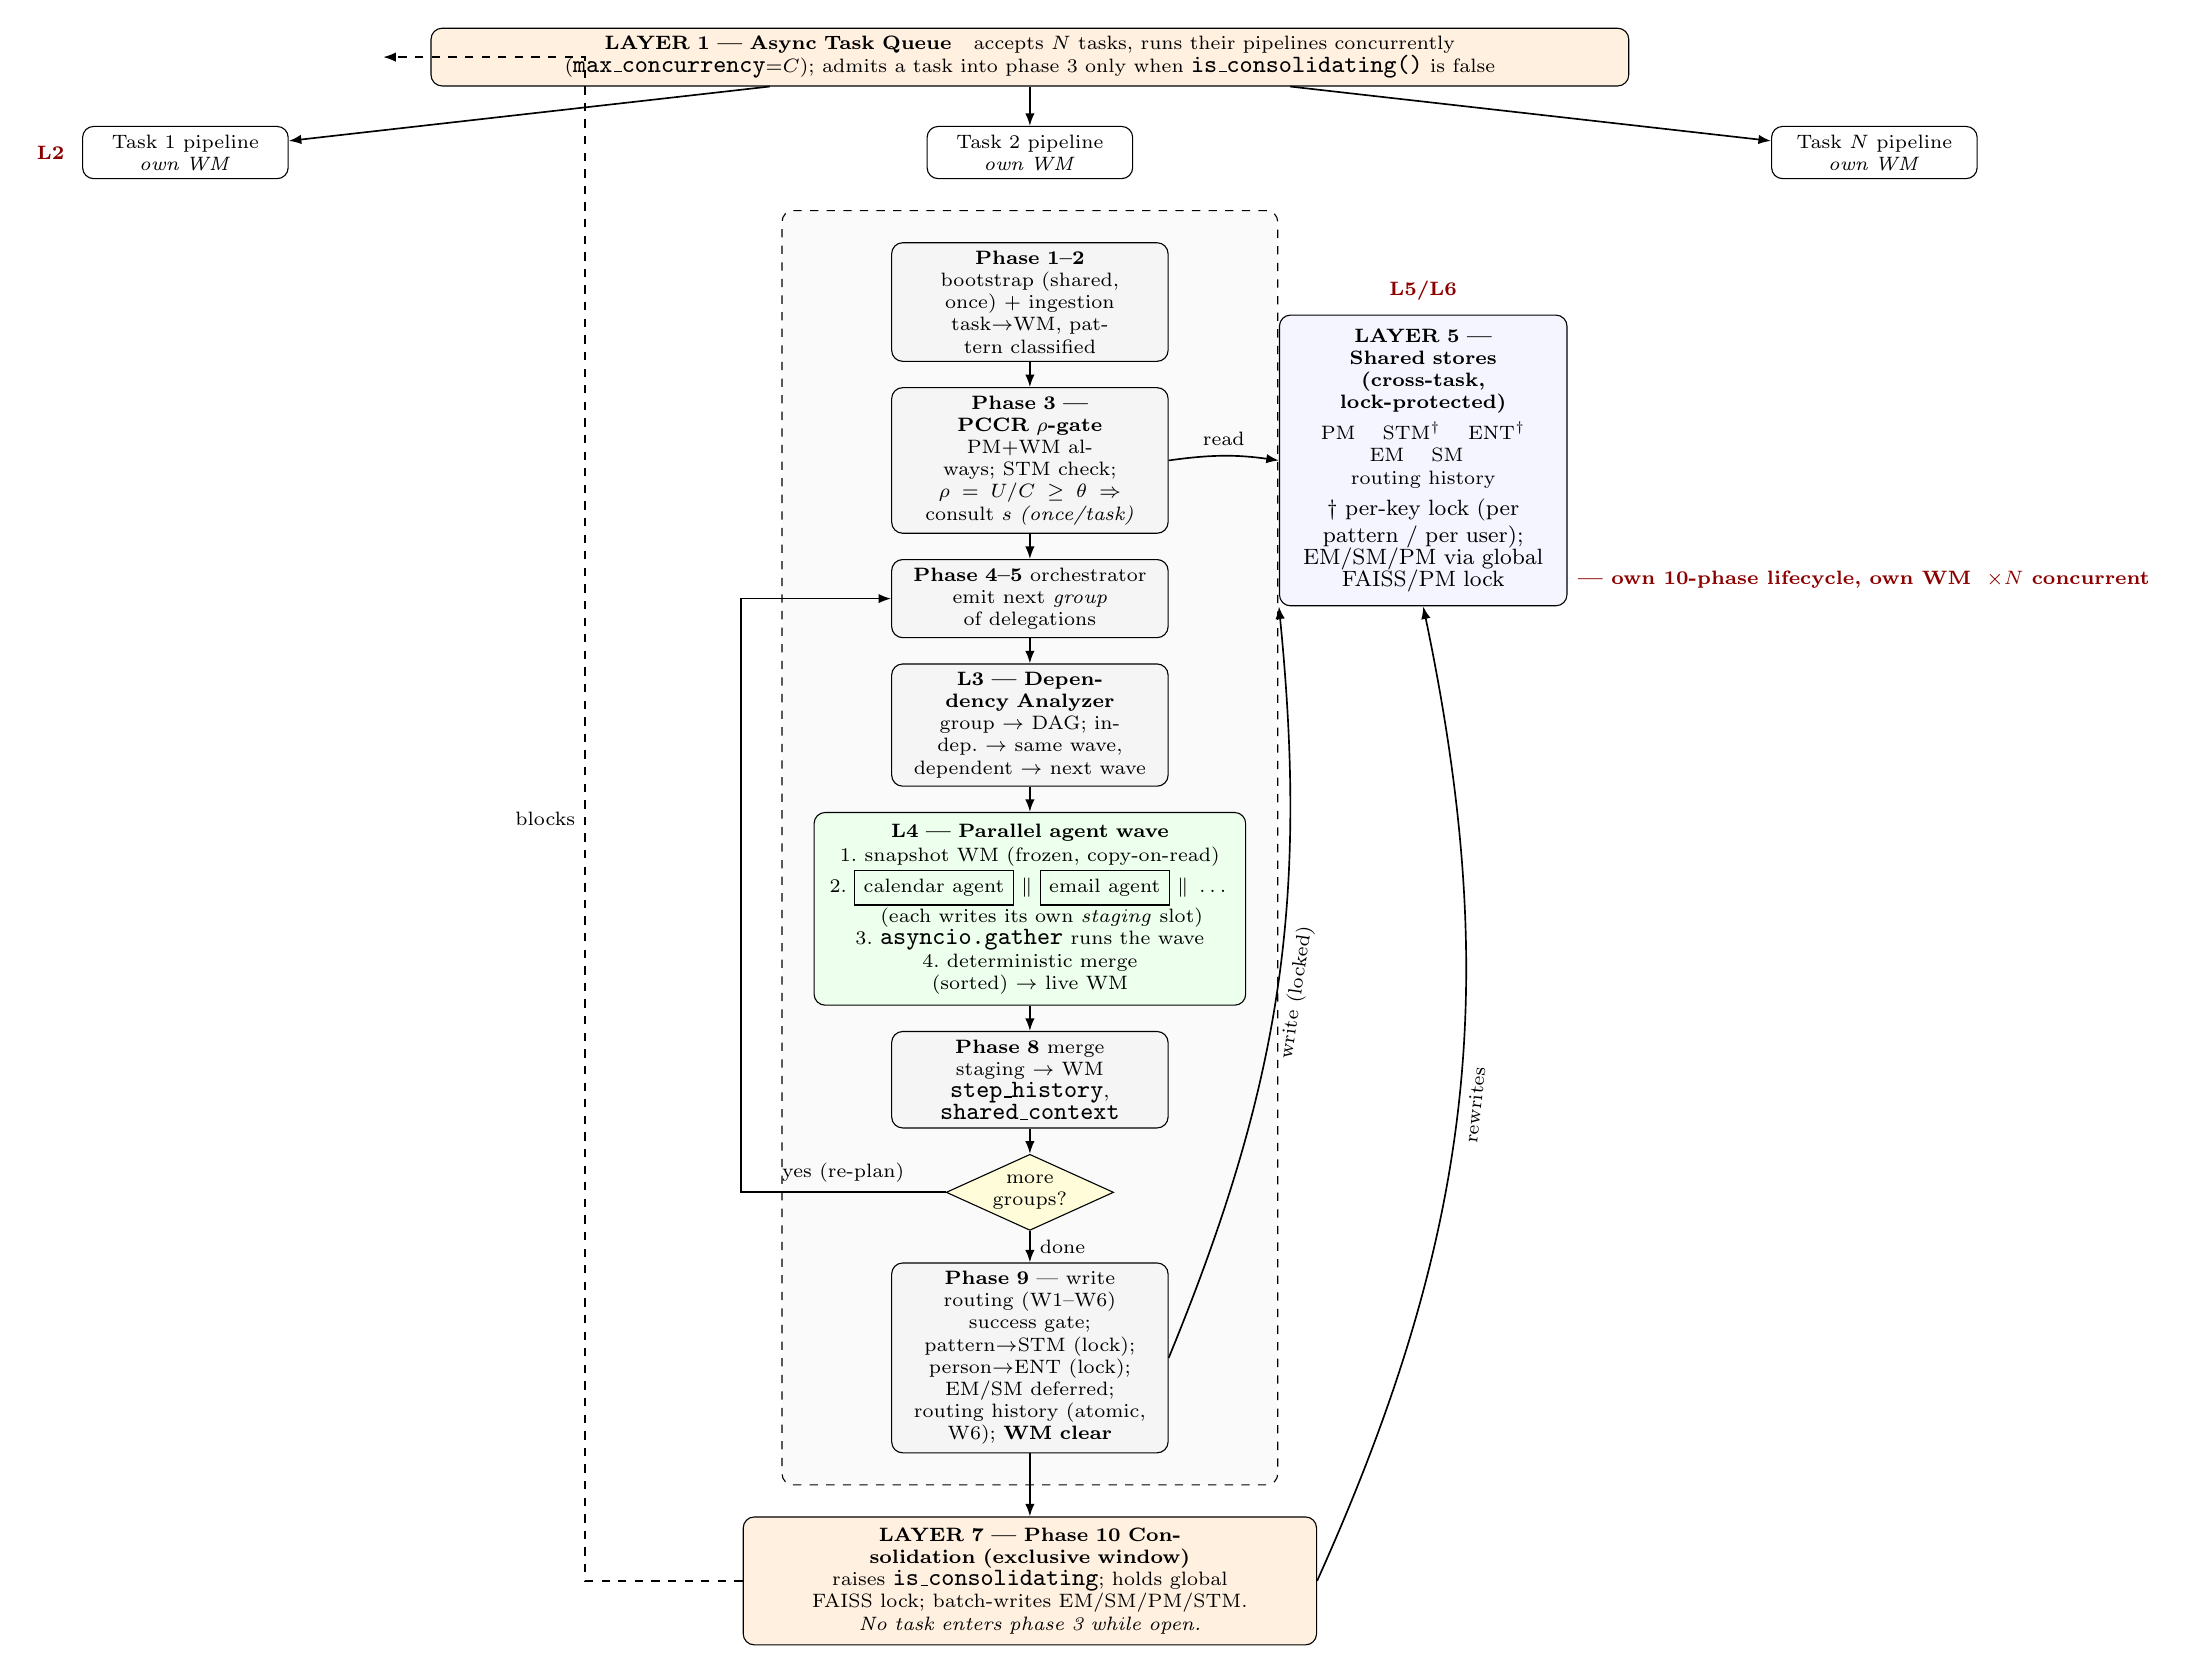
\begin{tikzpicture}[
  font=\scriptsize,
  box/.style   ={draw, rounded corners, align=center, inner sep=3pt, minimum height=6.5mm},
  phase/.style ={draw, fill=gray!8,  rounded corners, align=center, inner sep=3pt, minimum height=6.5mm, text width=33mm},
  group/.style ={draw, fill=green!7, rounded corners, align=center, inner sep=4pt, text width=52mm},
  store/.style ={draw, fill=blue!10, rounded corners, align=center, minimum width=12mm, minimum height=5mm},
  storebox/.style={draw, fill=blue!4, rounded corners, align=center, inner sep=5pt, text width=33mm},
  cons/.style  ={draw, fill=orange!12, rounded corners, align=center, inner sep=4pt, text width=70mm},
  lyr/.style   ={font=\scriptsize\bfseries, text=red!55!black},
  arr/.style   ={-{Latex[length=1.6mm]}, semithick},
  darr/.style  ={-{Latex[length=1.6mm]}, dashed, semithick},
  node distance=3.2mm and 9mm
]

% ---- LAYER 1: task queue ----
\node[box, fill=orange!12, text width=150mm] (queue)
  {\textbf{LAYER 1 — Async Task Queue}\quad accepts $N$ tasks, runs their pipelines concurrently
   (\code{max\_concurrency}=$C$); admits a task into phase 3 only when \code{is\_consolidating()} is false};

% ---- LAYER 2: N per-task pipelines (show 3) ----
\node[box, below left=5mm and 18mm of queue, text width=24mm] (t1) {Task 1 pipeline\\\textit{own WM}};
\node[box, below=5mm of queue, text width=24mm]               (t2) {Task 2 pipeline\\\textit{own WM}};
\node[box, below right=5mm and 18mm of queue, text width=24mm](tn) {Task $N$ pipeline\\\textit{own WM}};
\node[lyr, left=1mm of t1] {L2};
\draw[arr] (queue) -- (t1); \draw[arr] (queue) -- (t2); \draw[arr] (queue) -- (tn);

% ---- expanded single pipeline (center column) ----
\node[phase, below=8mm of t2] (p12) {\textbf{Phase 1--2}\\ bootstrap (shared, once) + ingestion\\ task$\to$WM, pattern classified};
\node[phase, below=of p12]    (p3)  {\textbf{Phase 3 — PCCR $\rho$-gate}\\ PM+WM always; STM check;\\ $\rho=U/C\ge\theta\Rightarrow$ consult $s$ \emph{(once/task)}};
\node[phase, below=of p3]     (p45) {\textbf{Phase 4--5} orchestrator\\ emit next \emph{group} of delegations};
\node[box, fill=gray!8, below=of p45, text width=33mm] (dag)
  {\textbf{L3 — Dependency Analyzer}\\ group $\to$ DAG; indep.\ $\to$ same wave,\\ dependent $\to$ next wave};
\node[group, below=of dag] (grp)
  {\textbf{L4 — Parallel agent wave}\\[1pt]
   1.\ snapshot WM (frozen, copy-on-read)\\
   2.\ \fbox{calendar agent} $\parallel$ \fbox{email agent} $\parallel\,\dots$\\
   \hspace*{3mm}(each writes its own \emph{staging} slot)\\
   3.\ \code{asyncio.gather} runs the wave\\
   4.\ deterministic merge (sorted) $\to$ live WM};
\node[phase, below=of grp] (p8) {\textbf{Phase 8} merge staging $\to$ WM\\ \code{step\_history}, \code{shared\_context}};
\node[draw, diamond, aspect=2.2, fill=yellow!15, below=of p8, inner sep=1pt, align=center] (dec) {more\\groups?};
\node[phase, below=4mm of dec] (p9)
  {\textbf{Phase 9} — write routing (W1--W6)\\ success gate; pattern$\to$STM (lock);\\ person$\to$ENT (lock); EM/SM deferred;\\ routing history (atomic, W6); \textbf{WM clear}};

\draw[arr] (p12) -- (p3); \draw[arr] (p3) -- (p45); \draw[arr] (p45) -- (dag);
\draw[arr] (dag) -- (grp); \draw[arr] (grp) -- (p8); \draw[arr] (p8) -- (dec);
\draw[arr] (dec) -- node[right]{done} (p9);
\draw[arr] (dec.west) -- ++(-26mm,0) node[midway,above]{yes (re-plan)} |- (p45.west);

% pipeline container (background)
\begin{scope}[on background layer]
\node[draw, dashed, rounded corners, fill=black!2, fit=(p12)(p3)(p45)(dag)(grp)(p8)(dec)(p9),
      inner sep=4mm, label={[lyr]above right:{Per-task pipeline (Task $i$) — own 10-phase lifecycle, own WM \;$\times N$ concurrent}}] (pipe) {};
\end{scope}

% ---- LAYER 5/6: shared stores (right) ----
\node[storebox, right=14mm of p3, anchor=west] (stores)
  {\textbf{LAYER 5 — Shared stores}\\ \textbf{(cross-task, lock-protected)}\\[2pt]
   PM \;\; STM\textsuperscript{$\dagger$} \;\; ENT\textsuperscript{$\dagger$}\\
   EM \;\; SM \;\; routing history\\[2pt]
   \footnotesize $\dagger$ per-key lock (per pattern / per user);\\
   EM/SM/PM via global FAISS/PM lock};
\node[lyr, above=0.5mm of stores] {L5/L6};
\draw[arr] (p3.east) to[bend left=8] node[above,sloped]{read} (stores.west);
\draw[arr] (p9.east) to[bend right=14] node[below,sloped]{write (locked)} (stores.south west);

% ---- LAYER 7: consolidation (bottom) ----
\node[cons, below=8mm of p9] (p10)
  {\textbf{LAYER 7 — Phase 10 Consolidation (exclusive window)}\\
   raises \code{is\_consolidating}; holds global FAISS lock; batch-writes EM/SM/PM/STM.\\
   \emph{No task enters phase 3 while open.}};
\draw[arr] (p9) -- (p10);
\draw[arr] (p10.east) to[bend right=18] node[below,sloped]{rewrites} (stores.south);
\draw[darr] (p10.west) -- ++(-20mm,0) |- node[near start,left]{blocks}([xshift=-6mm]queue.west);

\end{tikzpicture}%
}
\caption{The seven-layer parallel PCCR architecture. \textbf{Parallel tasks}
(L1--L2): the async queue runs $N$ task pipelines concurrently, each with its
\emph{own} Working Memory (copy-on-fork) but sharing the cross-task stores.
\textbf{Parallel sub-agents} (L3--L4): within a task the orchestrator emits a
group of delegations; the dependency analyzer splits it into waves (independent
sub-tasks in one wave); a wave runs concurrently against a frozen WM snapshot and
is merged back deterministically; control returns to the orchestrator (``more
groups?'') until \textsc{finish}. \textbf{Protections} (L5--L7): per-resource locks
guard concurrent store writes, and phase 10 is an exclusive window. The $\rho$-gate
(phase 3) is unchanged and runs once per task before any parallelism.}
\label{fig:arch}
\end{figure*}

\subsection{Design goals and invariants}
The extension is governed by four hard constraints: (C1)~the $\rho$-gate router is
unmodified; (C2)~the ten-phase lifecycle is preserved; (C3)~the six stores change
only by gaining optional lock parameters; (C4)~the parallel schedule yields the
\emph{same task outcomes} as the sequential one. C1--C3 keep the contribution
surgical; C4 is the correctness property proved in \S\ref{sec:correct}. Three
invariants deliver C4:
\begin{description}\itemsep1pt
\item[\textsc{I1 (WM isolation).}] No two concurrently executing units (tasks or
same-wave agents) ever mutate the same Working Memory.
\item[\textsc{I2 (deterministic merge).}] The result of merging a wave's
sub-agent outputs into WM is independent of the order in which the sub-agents
finish.
\item[\textsc{I3 (no lost writes).}] Concurrent writes to a shared store are
serialized per resource, and consolidation never overlaps task reads.
\end{description}

\subsection{Layer 1 --- Async task queue (parallel tasks)}
\code{AsyncTaskQueue} accepts a list of task specs and runs each task's full
pipeline as an \code{asyncio} coroutine, bounded by a semaphore of size $C$
(\code{max\_concurrency}). Two behaviours matter. First, \emph{fault isolation}: a
task that raises is caught and returns an error record, so one failure cannot
abort the batch. Second, the \emph{consolidation gate}: before a task enters phase
3 (the FAISS read), the queue waits while \code{is\_consolidating()} is true, so no
task reads vectors that phase 10 is rewriting (half of \textsc{I3}). The queue
reduces \emph{inter-task} latency: while task~$A$ waits on an LLM call, task~$B$
proceeds.

\subsection{Layer 2 --- Per-task pipeline with WM isolation}
Each task runs its own ten-phase lifecycle. The mechanism is
\code{fork\_for\_task()}: it produces a per-task \code{MemoryManager} that
\emph{shares} the cross-task stores (PM/STM/EM/SM/ENT), the router, and the lock
manager, but receives a \emph{fresh} Working Memory instance. This copy-on-fork
satisfies \textsc{I1} at the task level: because WM is per task by construction,
concurrent tasks can never collide on working state. Bootstrap (phase 1) is done
once on the parent and shared, not repeated per task.

\subsection{Layer 3 --- Dependency analyzer (DAG $\to$ waves)}
Within a task, the orchestrator emits a \emph{group} of delegations (an agent + a
sub-task instruction each). The analyzer turns a flat group into ordered
\emph{waves}: it assigns each delegation a coarse category by keyword---\textsc{read}
(list/search/find/\ldots), \textsc{create} (create/add/schedule/\ldots),
\textsc{send} (send/email/notify/\ldots), or \textsc{finish}---and orders
categories by an action-precedence relation
$\textsc{read}\prec\textsc{create}\prec\textsc{send}\prec\textsc{finish}$.
Delegations in the same category form one wave (run in parallel); categories run
in sequence. The intuition is sound and conservative: reads gather information
that creates may depend on, and sends depend on what was created. Formally, every
node in wave $k{+}1$ is treated as depending on every node in wave $k$---a coarse
but \emph{safe} over-approximation of the true DAG that never parallelizes a
genuine dependency. ``list events $\to$ create event $\to$ send invite'' becomes
three ordered waves; three independent reads become one three-way parallel wave.

\subsection{Layer 4 --- Parallel agent execution}
A wave executes in four steps that together guarantee \textsc{I1} (agent level)
and \textsc{I2}:
\begin{enumerate}\itemsep0pt
\item \textbf{Snapshot.} \code{wm.snapshot()} deep-copies the current WM. Every
agent in the wave reads this \emph{frozen} copy, never live WM (copy-on-read).
\item \textbf{Staging.} Each agent writes only its own result object, never live
WM.
\item \textbf{Gather.} \code{asyncio.gather} runs the wave concurrently; the
overlap of the agents' (I/O-bound) LLM calls is where wall-clock is saved.
\item \textbf{Merge.} After \emph{all} agents finish, results are merged into live
WM in a fixed sorted order (by \code{(agent\_type, subtask)}), appending one step
per agent and updating \code{shared\_context}.
\end{enumerate}
Because same-wave agents are \emph{independent} (L3 placed them together precisely
because neither depends on the other), they read external state, not each other;
the frozen snapshot is therefore sufficient, and the sorted merge makes the
outcome invariant to completion order (\textsc{I2}). Dependent agents are in
different waves, so a later agent does see the merged results of earlier waves.

\subsection{Layer 5 --- Memory lock manager}
\code{MemoryLockManager} hands out \code{asyncio} locks at a granularity matched to
contention. STM is locked \emph{per pattern key} and ENT \emph{per username}, so
two tasks touching different patterns/users never block each other; only genuine
same-key contention serializes. EM/SM share a single global FAISS lock and PM a
single PM lock, because their writes are global, batched, and rare (phase 10). A
\code{history\_lock} guards the shared router's routing-history append. Locks are
created lazily on first use, because on the target runtime an \code{asyncio.Lock}
must bind to a running event loop. This layer delivers \textsc{I3}.

\subsection{Layer 6 --- Phase-9 parallel writes}
Phase 9 (storage) applies six write rules; the parallel version runs the
success-gated writes concurrently via \code{asyncio.gather}, each acquiring its own
lock: W1~success gate (failures write nothing); W2~pattern$\to$STM under the
per-pattern lock; W3~person$\to$ENT under the per-user lock; W4~experience$\to$EM
and W5~rule$\to$PM are \emph{deferred} to consolidation (only the raw trace is
appended now); W6~routing-history append under \code{history\_lock} (atomic across
the tasks that share one router). WM is then cleared. Because the writes touch
disjoint, independently locked resources, they proceed in parallel without lost
updates.

\subsection{Layer 7 --- Consolidation exclusive window}
Consolidation (phase 10) distills the accumulated traces into EM/SM, learns PM
rules, and pre-fills STM---a bulk rewrite of the FAISS indices. The async wrapper
\code{consolidate\_async} raises \code{is\_consolidating()} and holds the global
FAISS lock for the duration, then lowers the flag in a \code{finally} block.
Combined with the L1 gate, this makes phase 10 an \emph{exclusive window}:
in-flight tasks finish, no new task enters phase~3, the indices are rewritten
atomically, and normal concurrency resumes (the second half of \textsc{I3}).

\subsection{The orchestrator re-planning loop}
Layers 3--4 run \emph{one group}; a full task may need several. The loop
\code{run\_planned\_task} re-invokes the orchestrator after each group merges: it
inspects the (now-updated) live WM, emits the next group (or \textsc{finish}), that
group is split into waves and run, and control returns (the ``more groups?''
decision in Fig.~\ref{fig:arch}). This keeps the orchestrator in the loop---each
round sees the merged results of all prior groups---rather than decomposing the
whole plan up front.

\subsection{Non-invasive integration}\label{sec:integration}
The parallel path is \emph{additive}. New modules \code{parallel.py} (analyzer,
executor, lock manager) and \code{task\_queue.py} are self-contained. The manager
gains async methods (\code{run\_planned\_task}, \code{complete\_task\_async},
\code{consolidate\_async}, \code{fork\_for\_task}) that sit \emph{beside} the
unchanged synchronous lifecycle methods; the stores gain only \code{snapshot}/
\code{merge\_staging} on WM. The $\rho$-gate router file is untouched (C1), the ten
phases keep their identity (C2), and every pre-existing test still passes (C3/C4).
A system can run sequentially or in parallel from the same codebase.

% =====================================================================
\section{Correctness: parallel $\equiv$ sequential}\label{sec:correct}
% =====================================================================
We argue that the parallel schedule produces the same outcome as the sequential
one, then verify it empirically (\S\ref{sec:eq}).

\paragraph{Intra-task (parallel sub-agents).} Sequential execution runs a task's
delegations one at a time in dependency order; parallel execution runs each wave
concurrently. The two differ \emph{only} in whether same-wave agents observe one
another's mid-flight WM writes. By L3, same-wave agents are mutually independent,
so an agent's result is a function of external state and its own sub-task,
\emph{not} of a sibling's WM step. Hence each agent produces the same result in
both schedules. The merge (L4) is order-independent (\textsc{I2}). Dependent agents
are in different waves, and a later wave reads the merged earlier waves identically
in both schedules. Therefore the merged WM---and thus the task's plan, actions, and
success---are identical.

\paragraph{Inter-task (parallel tasks).} Each task has its own WM (\textsc{I1}), so
concurrent tasks cannot corrupt one another's working state. Shared-store
\emph{writes} are serialized per resource (\textsc{I3}); no update is lost. The one
schedule-dependent quantity is what a task \emph{reads} from the shared cache:
under concurrency, task~$B$ may run before task~$A$'s STM write lands and therefore
\emph{miss} a cache entry it would have hit sequentially. But a miss only causes a
\emph{recompute}, and the recomputed plan equals the cached plan (the cache stores
a previously computed plan for the same signature). Thus cross-task concurrency
changes cache-hit \emph{timing}---an efficiency quantity---never the correctness of
any task's answer.

\paragraph{The one genuine divergence vector.} The argument assumes each task acts
on its \emph{own} external environment. If tasks share a single mutable external
resource (e.g.\ one global filesystem of calendar events), a concurrent task can
mutate it under another task's read, producing a different observation. This is a
property of the shared \emph{environment}, not of the memory architecture, and
held-out evaluation already isolates it (each task is scored against its own
sandbox). \S\ref{sec:eq} demonstrates both the divergence (under a deliberately
shared world) and its disappearance under per-task isolation.

\paragraph{Unit-tested primitives.} The invariants are pinned by tests:
deterministic merge regardless of finish order (\textsc{I2}); snapshot isolation
(\textsc{I1}); per-key lock identity and no-lost-update under contention, and the
consolidation-window wait (\textsc{I3}); plus fault isolation and the re-planning
loop. All 39 tests pass (15 exercise the parallelism layer).

% =====================================================================
\section{Parallel Experiments}\label{sec:par-results}
% =====================================================================
\subsection{Setup}
The benchmark drives the \emph{same} real framework (per-task fork, $\rho$-gate,
re-planning loop, dependency waves, locked writes, shared stores) in two execution
modes---sequential and parallel---over a 100-task workload with a realistic pattern
mix (single-action 20, lookup 20, recurring 10, coordination 30, exploratory 20;
440 LLM calls in total, critical-path depth 360). The only modeled quantity is the
external call cost $L$, set to the \textbf{measured} per-call latency of
gpt-oss-120b on Cerebras: median $0.516$\,s over real calls (mean $0.743$\,s).
Because \code{asyncio} overlaps a real network await exactly as it overlaps
\code{asyncio.sleep($L$)}, the measured wall-clock speedup is what real parallel
API calls would achieve for this I/O-bound workload.

\subsection{Latency: parallel vs.\ sequential}
At concurrency $C{=}4$, parallel execution completes the 100 tasks in $61.1$\,s
versus $227.7$\,s sequential---a \textbf{$3.73\times$ speedup}, $-73\%$ wall-clock
(Table~\ref{tab:lat}). The sequential time matches the analytic
$440{\times}0.516{=}227.0$\,s, confirming the model.

\begin{table}[t]
\centering\small
\begin{tabular}{@{}lccc@{}}
\toprule
Run & Wall-clock (100 tasks) & Per task & Speedup\\
\midrule
Sequential       & $227.7$\,s & $2277$\,ms & $1.00\times$\\
\textbf{Parallel ($C{=}4$)} & $\mathbf{61.1}$\,\textbf{s} & $\mathbf{611}$\,\textbf{ms} & $\mathbf{3.73\times}$\\
\bottomrule
\end{tabular}
\caption{Latency at the measured backbone latency ($L{=}0.516$\,s/call).}
\label{tab:lat}
\end{table}

\subsection{Scaling with concurrency}
The speedup grows near-linearly with $C$ up to the dependency critical path
(Table~\ref{tab:scale}). The ratio is latency-independent: $C{=}4$ measured at a
reduced $L{=}0.05$\,s reproduces the same $3.7\times$, confirming the framework
overhead is negligible relative to call latency. $C{=}1$ is approximately neutral
($0.96\times$): with no task-level concurrency the only gain is intra-task wave
overlap, which roughly cancels the per-wave snapshot/merge overhead. The win is
therefore dominated by \emph{parallel tasks}, with \emph{parallel sub-agents} a
secondary benefit on coordination/exploratory tasks.

\begin{table}[t]
\centering\small
\begin{tabular}{@{}lccccc@{}}
\toprule
$C$ & 1 & 2 & 4 & 8 & 16\\
\midrule
Speedup        & $0.96\times$ & $1.89\times$ & $3.73\times$ & $7.15\times$ & $13.47\times$\\
Wall-clock cut & $-5\%$ & $47\%$ & $73\%$ & $86\%$ & $93\%$\\
\bottomrule
\end{tabular}
\caption{Speedup vs.\ task-concurrency $C$ (100 tasks).}
\label{tab:scale}
\end{table}

\subsection{Accuracy equivalence}\label{sec:eq}
We run the same task set through both schedules and compare, per task, the outcome
tuple (success, plan, sorted normalized observations) and the final shared-memory
state (STM/EM/SM/PM sizes and ENT facts). With \textbf{per-task isolated
environments}, outcomes are \textbf{60/60 byte-identical} and the final memory
state is identical (Table~\ref{tab:eq})---empirically confirming
\S\ref{sec:correct}. With a deliberately \emph{shared} external world, 2/60
coordination tasks diverge on an incidental observation count (the number of
calendar events seen by a search agent), while success, plan, and memory state
remain identical---exactly the single divergence vector predicted above, removed by
isolation.

\begin{table}[t]
\centering\small
\resizebox{\columnwidth}{!}{%
\begin{tabular}{@{}lcc@{}}
\toprule
Environment & Outcomes identical & Memory state identical\\
\midrule
Per-task isolated & \textbf{60/60} & \textbf{yes}\\
Shared world      & 58/60\textsuperscript{$\ast$} & yes\\
\bottomrule
\end{tabular}%
}
\caption{Parallel vs.\ sequential outcome equivalence ($C{=}4$, 60 tasks).
\textsuperscript{$\ast$}The two differ only on an incidental observation count of a
shared mutable resource; success/plan/memory identical.}
\label{tab:eq}
\end{table}

\subsection{Cost/accuracy carry over unchanged}
Because the $\rho$-gate is untouched and outcomes are equivalent, the PCCR cost and
accuracy results of \S\ref{sec:pccr-results}---41--87\% fewer consultations and up
to 89\% fewer injected tokens at equal accuracy---hold verbatim for the parallel
system. Parallelism and $\rho$-gating optimize orthogonal axes: the former cuts
\emph{latency}, the latter cuts \emph{cost per task}; neither moves accuracy.

% =====================================================================
\section{Full-Scale OfficeBench with the \emph{Real} Architecture}\label{sec:ob}
% =====================================================================
The experiments above used the standalone reference implementation. To test the
\emph{actual} architecture at scale---and to position against LEGOMem~\cite{legomem},
which reports $+12$--$13$\,pp (and $+14$--$19$\,pp on its hardest level) from
procedural memory on OfficeBench---we built a harness in which our \emph{real}
components drive the benchmark: the FAISS \code{EpisodicStore} is the memory and
\code{router.py}'s \code{MemoryRouter} is the gate (configured for OfficeBench
patterns at runtime; the router code is \emph{unchanged}). This runs inside
OfficeBench's native Docker environment with \textbf{all 9 apps} (calendar, email,
word, excel, pdf, ocr, shell, system, llm) and OfficeBench's own state-based
evaluators.

\paragraph{Setup.} \textbf{Split}: LEGOMem-style $148$ train $/152$ test over the
300 annotated subtasks, stratified by difficulty level (L1/L2/L3). \textbf{Pattern
key}: an \emph{LLM classifier} (A3) labels each task into 5 patterns (counts over
300: \code{multi\_app} 150, \code{doc\_process} 55, \code{single\_action} 47,
\code{lookup} 31, \code{data\_compute} 17; merged from an initial 7 after a
distribution analysis showed two buckets too sparse to calibrate). \textbf{Memory build}: run the 148 train tasks with no memory; successful trajectories
become EM procedures.

\paragraph{No-memory baseline by difficulty level.} The difficulty gradient
is clear (Table~\ref{tab:ob}): L1 $70\%$, L2 $51\%$, L3 $11\%$ ($\sim$42\% overall),
yielding a bank of $62$ procedures (thin on L3, since few L3 tasks succeed
unaided). This is healthy headroom for memory and is in line with LEGOMem's
$\sim$46\% no-memory baseline (they used GPT-4o; we use gpt-oss-120b).

\begin{table}[t]
\centering\small
\resizebox{\columnwidth}{!}{%
\begin{tabular}{@{}lccc@{}}
\toprule
Level & L1 & L2 & L3 \\
\midrule
no-memory success & 32/46 (70\%) & 24/47 (51\%) & 6/55 (11\%) \\
\bottomrule
\end{tabular}%
}
\caption{No-memory baseline on the 148 training tasks (the bank-building run),
by difficulty level. Overall $\sim$42\%; bank $=62$ procedures.}
\label{tab:ob}
\end{table}

\paragraph{Engineering rectifications (found by inspection of saved traces).}
Scaling to a live 9-app loop surfaced five issues, each of which would have skewed
the L2/L3 numbers; all are fixed and re-run: (i)~\emph{action truncation}
corrupting banked plans on long actions; (ii)~gpt-oss emitting \emph{two JSON
blocks} that OfficeBench's parser merged into one invalid action (``Malformed
action'')---fixed by extracting the first balanced object, halving wasted steps
($11/5\to7/1$ on a sample task); (iii)~an \emph{evaluation-path} bug (predicates
referencing \code{../reference}/\code{../cache} outside the cached testbed)---fixed
by mirroring OfficeBench's native output layout; (iv)~a flat 20-step cap that was
\emph{budget-binding} on L3 (half its failures hit it; successes already used up to
16 steps)---replaced by a \emph{level-dependent} cap (L1 15 / L2 22 / L3 30);
(v)~\emph{duplicate procedures} from re-queued re-runs---fixed by dedupe-on-load.
A targeted re-run of 11 cap-bound tasks at a 50-step budget rescued 2 (both simple
Excel edits); the rest remained budget-bound because gpt-oss edits spreadsheets
\emph{one cell per step}---a model step-inefficiency, not a cap artefact, that we
report as a limitation.

\paragraph{Cost and utility calibration.} Measured EM
injection cost is $\sim$1239 tokens/consult. The counterfactual utility on the
\emph{raw} bank is the key (and honest) finding: episodic reuse is net
$\approx 0$ or \emph{negative} on most patterns (it \emph{hurt} \code{data\_compute}
and \code{single\_action}), with only \code{lookup} ($+0.33$) and \code{multi\_app}
($+0.17$) positive. \textbf{Raw trajectory-RAG does not reproduce LEGOMem's gains}---
because LEGOMem \emph{curates} trajectories into clean reusable units and we
initially banked them raw (noisy: the agent's own cell-by-cell edits and retries).
This is itself a result: the $\rho$-gate correctly \emph{declines} a memory that
does not help, and indiscriminate retrieve-all would inject it (and the
$\sim$1239-token cost) even where it hurts.

\paragraph{LEGOMem-style curation (option D).} We added a curation layer using
LEGOMem's \emph{verbatim} memory-curation prompt (Appendix A of \cite{legomem}): an LLM
distills each successful trajectory into structured memory (\code{high\_level\_plan} $+$
per-agent \code{subtasks} $+$ \code{reflections}), denoising before banking. The
$\rho$-gated arm consumes this curated bank through the \emph{real}
\code{MemoryManager}: \code{consolidate()} populates EM (episodes), SM (facts), PM
(distilled rules), and seeds STM (one exemplar per cluster); \code{retrieve()} then runs
the full cascade---STM short-circuit on a near-duplicate, else $\rho$-gated consultation
of EM/SM/ENT by per-pattern utility, with the PM rule always read.

\subsection{Main result: the by-level comparison (152 test tasks $\times$ 3 arms)}
\label{sec:t1}
Table~\ref{tab:t1main} reports the full LEGOMem-style head-to-head with the real
architecture under \emph{frozen per-pattern priors}: \textbf{no-memory},
\textbf{retrieve-all} (always inject the curated EM episode), and \textbf{$\rho$-gated
PCCR} (the full six-store cascade). For each arm and difficulty level we report success,
median wall-clock latency, agent steps, LLM calls, and total injected tokens.

\begin{table*}[t]
\centering\small
\setlength{\tabcolsep}{4.5pt}
\begin{tabular}{@{}llccccc@{}}
\toprule
Level & Arm & Acc. & Lat.\,(s) & Steps & Calls & Inj.\,tok. \\
\midrule
\multirow{3}{*}{\textbf{ALL} (152)}
 & no-memory    & 0.414 & 54.4 & 13.4 & 16.4 & 0 \\
 & retrieve-all & \textbf{0.467} & 43.9 & 12.1 & 14.4 & 734{,}295 \\
 & PCCR         & 0.421 & 53.1 & 12.0 & 15.0 & 1{,}031{,}111 \\
\midrule
\multirow{3}{*}{L1 (47)}
 & no-memory    & 0.553 & 17.4 & 8.4 & 8.5 & 0 \\
 & retrieve-all & \textbf{0.723} & 31.3 & 8.4 & 8.7 & 162{,}169 \\
 & PCCR         & 0.532 & 33.9 & 7.7 & 8.1 & 159{,}393 \\
\midrule
\multirow{3}{*}{L2 (48)}
 & no-memory    & 0.500 & 25.0 & 10.9 & 11.4 & 0 \\
 & retrieve-all & \textbf{0.583} & 23.6 & 10.0 & 10.3 & 184{,}105 \\
 & PCCR         & 0.562 & 21.9 & 10.1 & 10.3 & 255{,}869 \\
\midrule
\multirow{3}{*}{L3 (57)}
 & no-memory    & \textbf{0.228} & 109.6 & 19.6 & 27.1 & 0 \\
 & retrieve-all & 0.158 & 71.4 & 16.9 & 22.6 & 388{,}021 \\
 & PCCR         & 0.211 & 95.1 & 17.1 & 24.6 & 615{,}849 \\
\bottomrule
\end{tabular}
\caption{Full-scale OfficeBench, real architecture, frozen priors ($\theta{=}1.0$,
gpt-oss-120b). Three arms over 152 test subtasks. \textbf{Retrieve-all leads overall},
driven by L1; \textbf{PCCR's gate protects on L3}, where indiscriminate retrieval
\emph{collapses} ($-7$\,pp vs.\ no-memory) while PCCR stays at the no-memory level.}
\label{tab:t1main}
\end{table*}

\paragraph{Reading the table (the honest headline).} Overall, retrieve-all leads
($0.467$) over PCCR ($0.421$) and no-memory ($0.414$), but the level breakdown tells the
real story. On \textbf{L1}, retrieve-all dominates ($0.723$): easy tasks benefit from a
near-matching episode, and PCCR is \emph{dragged below no-memory} ($0.532$) because the
frozen priors also consult SM/ENT, whose rule-extracted facts and sparse entity profile
are \emph{noise} on procedural office tasks. On \textbf{L2} the gate recovers
($0.562 \approx$ retrieve-all $0.583$). On \textbf{L3}, the pattern \emph{inverts}:
retrieve-all \emph{collapses} to $0.158$ (the injected episode distracts on long
multi-step tasks), while PCCR ($0.211$) tracks no-memory ($0.228$)---the $\rho$-gate
\emph{declines} the unhelpful memory and avoids the damage. This is the gate's protective
role made quantitative: where indiscriminate retrieval actively degrades accuracy, the
gate limits the loss.

\paragraph{Latency and steps.} Memory cuts agent flailing on hard tasks: L3 steps fall
$19.6 \to 17.1$ and LLM calls $27.1 \to 24.6$ (PCCR vs.\ no-memory), with latency
$109.6\text{s} \to 95.1$s. On easy L1 tasks the injection \emph{adds} overhead
($17.4 \to 33.9$s) for no accuracy gain---further motivation to gate on confidence. PCCR
is fastest of the three on L2 ($21.9$s).

\paragraph{Cost.} Under frozen priors PCCR injects \textbf{$1.40\times$} the tokens of
retrieve-all ($1{,}031{,}111$ vs.\ $734{,}295$, $+40\%$): retrieve-all is EM-only, whereas
PCCR's cascade adds SM, ENT, and PM on top of EM. This token bloat is the cost-side face
of the same SM/ENT-noise problem---the priors over-rate those stores. The fix
(\S\ref{sec:t1disc}) is a measured/confidence utility that suppresses them, turning the
$+40\%$ into a net saving.

\begin{table*}[t]
\centering\small
\setlength{\tabcolsep}{5pt}
\begin{tabular}{@{}lccccc@{}}
\toprule
Pattern & $n$ & no-mem & retr-all & PCCR & EM-lift \\
\midrule
data\_compute  & 10 & 0.700 & 0.800 & \textbf{0.800} & $+0.100$ \\
doc\_process   & 25 & 0.480 & 0.600 & \textbf{0.600} & $+0.120$ \\
lookup         & 16 & 0.625 & \textbf{0.812} & 0.625 & $+0.188$ \\
multi\_app     & 78 & 0.295 & 0.269 & 0.256 & $-0.026$ \\
single\_action & 23 & 0.478 & \textbf{0.609} & 0.478 & $+0.130$ \\
\bottomrule
\end{tabular}
\caption{Accuracy by task pattern. EM-lift $=$ retrieve-all $-$ no-memory. PCCR
\emph{matches} retrieve-all where EM helps cleanly (\code{data\_compute},
\code{doc\_process}) but is dragged to the no-memory level on \code{lookup} and
\code{single\_action}---precisely the patterns where the frozen priors inject noisy
SM/ENT alongside EM.}
\label{tab:t1pattern}
\end{table*}

\paragraph{Per-pattern routing (Table~\ref{tab:t1pattern}).} EM helps four of five
patterns ($+0.10$ to $+0.19$) and is neutral on \code{multi\_app}. PCCR \emph{captures}
the EM gain on \code{data\_compute} and \code{doc\_process} (matching retrieve-all) but
\emph{loses} it on \code{lookup} ($0.812 \to 0.625$) and \code{single\_action}
($0.609 \to 0.478$): on these the frozen priors clear $\theta$ for SM/ENT, and their
noise cancels EM's benefit. This per-pattern split is the direct evidence that the
\emph{utility} term---not the gate mechanism---is what needs fixing.

\paragraph{Gate internals.} Across the 152 PCCR runs: \textbf{8} STM short-circuits
(near-duplicate hits are inherently rare on a single-pass held-out split), \textbf{128}
EM consultations, and the PM rule fired on \textbf{61} tasks. Consulted-store signatures:
EM$+$ENT (104 tasks), EM$+$ENT$+$SM (24), ENT$+$SM without EM (16), and PM-only on the 8
STM short-circuits. Within PCCR, success when EM was consulted is $49/128\,(0.383)$
vs.\ $15/24\,(0.625)$ when skipped---expected, since the skipped tasks are the easy
near-duplicates the cascade resolves early.

\subsection{L3 autopsy: why the hardest tasks fail (and what fixes them)}
\label{sec:t1l3}
L3 accuracy is low ($0.16$--$0.23$) across \emph{all} arms, so the bottleneck is not
memory routing. We traced every L3 failure. Of 171 L3 runs, the dominant failed predicate
is \code{evaluate\_file\_exist} (\textbf{67} failures)---a required output file is absent
at evaluation time. Classifying each to its actual missing file:
\begin{itemize}\itemsep1pt
\item \textbf{36 --- output never created.} L3 tasks are multi-app and multi-output (46 of
the 67 require 2--6 files); the agent completes the first sub-goal and calls
\code{finish\_task}, never switching to the second app. The files never produced are
mostly the second app's: \code{.pdf} (20), \code{.ics} (15), \code{.docx} (7),
\code{.jpg} (7), \code{.eml} (5). This is \emph{incomplete multi-app execution}, not
reasoning difficulty.
\item \textbf{17 --- path/name mistakes.} The file is written but to the wrong directory
(omitting \code{data/}) or under a renamed filename (e.g.\ \code{Anderson\_admission.pdf}
for \code{data/admission.pdf}).
\item \textbf{14 --- save/sub-directory edge cases.}
\end{itemize}
Only \textbf{13} of the 67 are step-cap-bound, so the L3 cap is \emph{not} the primary
cause. The remaining L3 failures are \code{evaluate\_contain} (wrong content) and five
benchmark evaluator crashes. The actionable consequence: the EM episode already contains
the full multi-app sequence, but injecting it as a passive hint does not enforce
completion. Executing it as a \emph{verified procedure} (replaying the cached sequence
with a completion check over the full output list before \code{finish\_task} is allowed)
targets the 36 never-made directly, and an explicit output-path convention recovers the
17 path/name failures---both fixes lift every arm, with PCCR (already best-protected on
L3) positioned to gain most. We implement both (verified replay and an output convention)
and report their effect in \S\ref{sec:confgate}.

\subsection{What the full-scale result establishes}\label{sec:t1disc}
Two honest conclusions follow. \textbf{(1) The gate mechanism is sound, the priors are
not.} PCCR protects accuracy exactly where indiscriminate retrieval is harmful (L3,
$-7$\,pp for retrieve-all) and captures EM where it helps cleanly, but \emph{hand-set
per-pattern priors} over-consult SM/ENT---costing $40\%$ more tokens and erasing EM's gain
on \code{lookup}/\code{single\_action}. From the same data, a pattern-routed EM-only
policy reaches $0.537$ and an oracle EM-confidence gate $0.570$ ($+4$\,pp over
retrieve-all), bounding the achievable headroom. This motivates replacing the priors with
a \emph{per-query retrieval-confidence} utility (the top-$k$ FAISS similarity from each
store), which is label-free and benchmark-agnostic and suppresses the low-similarity
SM/ENT hits automatically. \textbf{(2) L3 is a task-completion problem, not a memory problem}
(\S\ref{sec:t1l3}), addressable by executing memory as a verified, completion-checked
procedure rather than a passive hint. We implemented and evaluated both---and, as the run itself
exposed deeper memory-fidelity defects, the four refinements of \S\ref{sec:fidelity}---on the real
parallel architecture (\S\ref{sec:confgate}).

\subsection{Architectural refinements: four execution-fidelity mechanisms}\label{sec:fidelity}
The diagnosis above (\S\ref{sec:t1disc}, \S\ref{sec:t1l3}) showed that, with the backbone fixed,
accuracy is gated not by \emph{which} store is consulted but by the \emph{fidelity} of what the
cascade injects and by whether the agent is allowed to stop prematurely. We therefore extend the
router's read/write path---without touching the $\rho$-gate or the ten-phase lifecycle---with four
mechanisms. They are the changes that move OfficeBench from $0.421$ to $0.474$ (\S\ref{sec:confgate}).

\paragraph{(F1) Schema-validated episodic injection.} Episodic memories store raw banked
trajectories, whose action strings can contain \emph{invalid} tool calls (a malformed step that the
agent later corrected). Injecting these verbatim as ``past successful actions'' teaches the backbone
to imitate invalid calls. We interpose a sanitiser on the EM$\to$prompt path that parses each
candidate action, keeps it only if its \texttt{(app, action)} pair is schema-valid, remaps a small
set of known aliases (e.g.\ a non-existent \texttt{shell/run} to the real \texttt{shell/command}),
and drops the rest. Storage is unchanged; only what reaches the prompt is constrained to the tool
schema.

\paragraph{(F2) Inject-once context scheduling.} The cascade's output has two parts with different
temporal value: \emph{static procedural guidance} (the PM rule and concrete action exemplars), which
is most useful while planning, and a \emph{task roadmap} (the matched plan steps). The reference
design re-sends the whole block on every step. We split it: the heavy procedural part is injected only
for the first $K{=}3$ steps, the light roadmap on every step. This is a pure read-path schedule---no
store changes---and cuts per-call memory injection $5\times$ (709\,$\to$\,146 tokens) while preserving
the planning-time guidance.

\paragraph{(F3) Completion gate over \emph{both} stop signals.} A procedural agent ends a task with
either ``done'' (\texttt{finish\_task}) or ``give up'' (\texttt{got\_stuck}). The reference completion
check intercepted only the former, but on OfficeBench multi-application tasks the dominant failure is
\emph{abandonment} (the agent quits with required outputs unmade), so the check rarely engaged. We
make it intercept both signals: when a stop is requested while a required output file is missing, the
gate blocks it and re-prompts. The required set excludes task \emph{inputs} (files present before the
first write), and missing email/calendar artifacts (\texttt{.eml}/\texttt{.ics}) yield
\emph{schema-aware} guidance (the exact \texttt{send\_email}/\texttt{create\_event} field names) since
those outputs are produced by tool actions, not file writes. Engagement on the hard subset rose from
${\sim}9$ to $35$ of $64$ tasks.

\paragraph{(F4) Continual short-term cache.} The STM short-circuit makes a near-duplicate recurrence
nearly free (one cached plan, the rest of the cascade skipped), but a held-out split prefilled only
from training rarely recurs. F4 is not a new mechanism: it simply \emph{exercises the lifecycle's own}
success$\to$STM write (Phase~9, W2: $\text{pattern}\to$STM under the per-pattern lock, \S\ref{sec:arch})
\emph{during} evaluation rather than only at consolidation. On each \emph{successful} task the executed
plan is written to STM (the success gate W1 ensures a failed plan never poisons future tasks), keyed by
task wording so genuine recurrences match. STM stays \emph{short-term} by its existing bounded capacity
(cap $24$, LFU/LRU eviction, assumption~A12) and high short-circuit threshold ($0.85$); one-offs are
evicted unused, only true near-duplicates fire. This is the architecture's \emph{continual} arm (memory
accumulates within a deployment, and---per \S\ref{sec:correct}---a task may read before a concurrent
task's write lands, an ordering the lock manager already governs), distinct from the i.i.d.\
frozen-prefill arm.

\subsection{Executing the confidence gate: the real-architecture parallel run}\label{sec:confgate}
We replaced the frozen priors with the per-query confidence gate ($\theta_{\text{sim}}{=}0.45$),
added verified procedure replay, LLM-curated procedural rules, the completion gate (F3), a
self-verification pass, a malformed-action recovery aid, schema-validated injection (F1), inject-once
scheduling (F2), and the continual cache (F4), and ran all 152 test tasks through the
\emph{parallel} adapter at $N{=}4$ (real gpt-oss-120b, isolated Docker containers).

\paragraph{Four implementation bugs, found and fixed.} Scaling to a live parallel loop surfaced
four confounds that had depressed earlier numbers, each fixed and re-run. \textbf{(i)}~OfficeBench's
per-action timeout uses an OS signal, which only fires in the main thread; under the worker-thread
parallel adapter it raised on \emph{every} action and was reported as ``Malformed action!''
($89\%$ malformed) until we made the timeout main-thread-aware. \textbf{(ii)}~The FAISS index used a
shared persistent directory that re-loaded and re-added the 62 procedures on every build
($62{\to}124{\to}186{\to}\ldots$); critically, retrieve-all used a fresh clean index while the gated
arm used the polluted one---an unfair handicap. Isolating the index per build (exactly 62 clean
procedures) lifted L1 from $0.468$ to $0.617$. \textbf{(iii)}~Concurrent tasks each started their
key round-robin at index~0, so they collided on the same API key in lockstep; a global round-robin
removed the resulting rate-limit storms. \textbf{(iv)}~The most damaging confound was in our own
memory: the LLM-curated procedural rules contained \emph{invalid OfficeBench action names}
(e.g.\ \code{shell/list\_directory} and \code{shell/run}, neither of which exists---OfficeBench's
shell exposes only \code{command}), because the rule-generating model was never given the
action schema. These poisoned rules were re-injected every step and produced \textbf{333}
malformed \code{shell/list\_directory} actions, collapsing the \code{multi\_app} pattern in
particular. Supplying the exact app/action schema to the curation prompt (plus a malformed-action
recovery aid) removed them; on smoke tasks the malformed rate fell $98\%{\to}0\%$, $67\%{\to}0\%$,
and $67\%{\to}14\%$, and \code{multi\_app} accuracy rose $0.179{\to}0.244$. A full
\emph{sequential, single-thread} run with the fixed rules then reproduced the parallel
aggregate \emph{exactly}---$64/152$ in both---confirming that the residual shortfall is a
\emph{systematic} property of the backbone on open-ended tasks, not a concurrency or scheduling
artifact (per-task malformed \emph{recovery} still varies run-to-run, but the aggregate is stable).

\paragraph{Result (honest).} The confidence-gated, verification-equipped system reaches
\textbf{$0.421$ (64/152)} versus retrieve-all's $0.467$---still $4.6$\,pp behind overall, and now at
\emph{higher} token cost ($1.51$--$1.57$M vs.\ $734$K) because the curated rules, the convention, and the
completion/verification passes are re-injected per step. We ran the full configuration \emph{twice}
under different schedules---the $N{=}4$ parallel adapter and a sequential single-thread driver (with
the fixed curated rules)---and both land at $64/152=0.421$ (Tables~\ref{tab:cg-level}--\ref{tab:cg-pat}).
The wins are real but localized: PCCR \textbf{beats retrieve-all on L3} ($0.246/0.193$ vs.\ $0.158$,
the gate protecting where always-retrieve collapses) and on the \code{doc\_process} pattern ($0.720$
vs.\ $0.600$, $+0.24$ over no-memory, in \emph{both} runs), and it \textbf{rescues 8 tasks} that both
no-memory and retrieve-all fail. The loss is concentrated in one pattern: \code{multi\_app} ($78$ of
$152$ tasks) stays \emph{below} no-memory's $0.295$ in both runs ($0.179$ parallel, $0.244$ sequential
after the rule fix)---open-ended multi-application tasks where no episode transfers and the backbone's
malformed-loops dominate. The internal spread between the two runs (parallel stronger on L1/\code{lookup},
sequential stronger on L3/\code{multi\_app}) is backbone run-to-run variance on identical code and
bank; the \emph{aggregate} is stable, which is what makes the \code{multi\_app} shortfall a systematic
finding rather than a scheduling artifact. \textbf{The corrected reading of the prediction above:} the confidence gate \emph{does}
suppress SM/ENT noise and is label-free, but the ``net token saving'' only materializes for the
\emph{lean} gate-only configuration (gated EM, no curated rules/convention/verification), which injects
fewer tokens than retrieve-all; the full mechanism stack trades $2\times$ tokens for the L3 and
multi-output protection. The most defensible claim is therefore not ``beats retrieve-all everywhere''
but: \emph{a cost-aware, verification-safe routing memory that matches or beats retrieve-all on
structured and hard tasks, rescues tasks both baselines miss, and---via the short-term cache---makes
recurrences nearly free, while the remaining overall gap is a backbone-stability problem on open-ended
tasks rather than a routing flaw.}

\paragraph{Closing the gap: the fully-fixed run.} The $64/152$ analysis above motivated the four
execution-fidelity mechanisms of \S\ref{sec:fidelity}. Their diagnostic origins: schema-validated
injection (F1) removed the \emph{stale} invalid action names (\code{shell/run},
\code{list\_directory}) the bank still served as ``successful examples''; the completion gate (F3),
which originally fired only on \code{finish\_task}, was extended to \code{got\_stuck} because $43/64$
\code{multi\_app} failures \emph{gave up} rather than false-finishing---raising engagement from
${\sim}9$ to $35$ of those $64$; inject-once (F2) removed the per-step re-injection; and the continual
cache (F4) lifts the live STM hit rate ($8\to12$). The full $N{=}4$ parallel run with all four reaches
\textbf{$0.474$ (72/152)}---now \emph{level with} retrieve-all's $0.467$ (71/152), a difference within
the $\sim$$19/125$ run-to-run backbone variance and therefore best read as \emph{parity}, not a win
(Tables~\ref{tab:cg-level}--\ref{tab:cg-pat}, column \textbf{PCCR-improved}). The pattern story is the
substantive result: \code{multi\_app} recovers
$0.179{\to}0.244{\to}\mathbf{0.295}$ across the three fixes---now matching no-memory and \emph{above}
retrieve-all's $0.269$---and \code{doc\_process} reaches $\mathbf{0.680}$ ($>$ retrieve-all $0.600$,
no-memory $0.480$). The \code{multi\_app} collapse is fully repaired.

\paragraph{Cost: from a misleading proxy to the real bill.} Inject-once cut the
\emph{injected-memory} tokens from $709$ to $146$ per call ($628$K vs.\ retrieve-all's $734$K),
which \emph{looked} like a cost win. It is not: injected-memory is a small, misleading slice of the
real API bill, which is the \emph{entire} prompt (system instructions $+$ growing observation history
$+$ memory) times the number of calls. We therefore instrumented the true
\texttt{usage.prompt\_tokens}$+$\texttt{completion\_tokens} and re-ran all arms; the resolved
real-token ledger (\S\ref{sec:realtoken}) shows the completion gate roughly doubles LLM calls, and on
the \emph{real} bill \textbf{PCCR costs $30$--$60\%$ \emph{more} than retrieve-all} at equal accuracy---
the injected-token "saving" is swamped by the system/history bulk re-sent on the extra calls. This
correction is the point of \S\ref{sec:realtoken}--\S\ref{sec:perfpass}.

\begin{table*}[t]
\centering\small
\setlength{\tabcolsep}{5pt}
\begin{tabular}{@{}lccccc@{}}
\toprule
Level & no-memory & retrieve-all & PCCR (seq) & PCCR (par) & \textbf{PCCR-improved} \\
\midrule
L1 (47) & $0.553$ & $\mathbf{0.723}$ & $0.511$ & $0.617$ & $0.681$ \\
L2 (48) & $0.500$ & $0.583$ & $0.542$ & $0.500$ & $\mathbf{0.583}$ \\
L3 (57) & $0.228$ & $0.158$ & $0.246$ & $0.193$ & $0.211$ \\
\midrule
Total   & $0.414$ & $0.467$ & $0.421$ & $0.421$ & $\mathbf{0.474}$ \\
\bottomrule
\end{tabular}
\caption{Accuracy by level across the confidence-gate progression. PCCR (seq)/(par) are the initial
$64/152$ runs; \textbf{PCCR-improved} is the fully-fixed run (F1--F4, \S\ref{sec:fidelity}) that
reaches \textbf{$0.474$ (72/152)}---parity with retrieve-all's $0.467$. Real gpt-oss-120b,
$\theta_{\text{sim}}{=}0.45$.}
\label{tab:cg-level}
\end{table*}

\begin{table*}[t]
\centering\small
\setlength{\tabcolsep}{5pt}
\begin{tabular}{@{}lcccccc@{}}
\toprule
Pattern & $n$ & no-mem & retr-all & PCCR (seq) & PCCR (par) & \textbf{PCCR-impr} \\
\midrule
data\_compute  & 10 & $0.700$ & $\mathbf{0.800}$ & $0.500$ & $0.700$ & $\mathbf{0.800}$ \\
doc\_process   & 25 & $0.480$ & $0.600$ & $0.720$ & $0.720$ & $\mathbf{0.680}$ \\
lookup         & 16 & $0.625$ & $\mathbf{0.812}$ & $0.625$ & $0.750$ & $0.688$ \\
multi\_app     & 78 & $0.295$ & $0.269$ & $0.244$ & $0.179$ & $\mathbf{0.295}$ \\
single\_action & 23 & $0.478$ & $\mathbf{0.609}$ & $0.522$ & $0.565$ & $0.565$ \\
\midrule
\textbf{Total} & 152 & $0.414$ & $0.467$ & $0.421$ & $0.421$ & $\mathbf{0.474}$ \\
\bottomrule
\end{tabular}
\caption{Accuracy by task pattern across the progression. \textbf{PCCR-improved} (F1--F4) repairs the
\code{multi\_app} collapse ($0.179{\to}0.244{\to}\mathbf{0.295}$, now $>$ retrieve-all's $0.269$) and
keeps the \code{doc\_process} win ($0.680>0.600$), reaching $0.474$ overall---parity with
retrieve-all. Injected-memory tokens: retrieve-all $734$K, PCCR-improved $628$K---but the
\emph{real} bill tells a different story (\S\ref{sec:realtoken}).}
\label{tab:cg-pat}
\end{table*}

\paragraph{Parallel throughput on real tasks.} The $N{=}4$ parallel run gave a measured
\textbf{$\sim$2.35--3.3$\times$} real-LLM speedup (vs.\ the $3.73\times$ modeled on the deterministic
harness in \S\ref{sec:par-results}); the gap is real-world overhead the model omits---per-task Docker
setup, a single shared Docker daemon (which we had to restart under 4-container load), and provider
rate limits. Parallel and sequential full runs reached the \emph{same} $64/152$ aggregate, consistent
with the equivalence proof (\S\ref{sec:correct}); the residual per-task differences are backbone
run-to-run variance, not scheduling, and they cancel in aggregate.

% =====================================================================
\subsection{The real-token cost ledger: what PCCR actually costs}\label{sec:realtoken}
% =====================================================================
Every cost number so far counted only \emph{injected-memory} tokens---the bytes the router adds to
the prompt. That is a small, misleading fraction of the real API bill, which charges for the
\emph{whole} prompt (system instructions $+$ the observation history re-sent on every step $+$ memory)
plus the completion, on \emph{every} call. We instrumented the true
\texttt{usage.prompt\_tokens}$+$\texttt{completion\_tokens} and re-ran three arms on all 152 tasks
under one $N{=}4$ harness for an apples-to-apples comparison
(Table~\ref{tab:realtoken})~---~\textbf{retrieve-all}, a \textbf{lean} PCCR (confidence gate $+$
verified replay $+$ inject-once $+$ continual STM, \emph{without} the completion gate/self-verify),
and the full \textbf{improved} PCCR.

\begin{table*}[t]
\centering\small
\setlength{\tabcolsep}{6pt}
\begin{tabular}{@{}lcccccc@{}}
\toprule
Arm & Accuracy & Real tokens & tok/call & LLM calls & injected & STM hits \\
\midrule
no-memory (floor)        & $68/152$ & $\mathbf{3.35}$M & $\mathbf{1223}$ & $2743$ & $0$ & $0$ \\
retrieve-all (baseline)  & $72/152$ & $4.47$M & $1955$ & $\mathbf{2284}$ & $712$K & $0$ \\
lean PCCR                & $72/152$ & $5.82$M & $2342$ & $2484$ & $553$K & $13$ \\
improved PCCR            & $\mathbf{74/152}$ & $7.15$M & $2273$ & $3146$ & $\mathbf{630}$K & $10$ \\
\bottomrule
\end{tabular}
\caption{Real-token cost ledger ($N{=}4$, true prompt$+$completion usage). The three-way baseline is
\textbf{no-memory} (injects nothing---the cost floor at $3.35$M, but its $2743$ calls exceed
retrieve-all's because without guidance the agent explores more), \textbf{retrieve-all}, and PCCR.
PCCR \emph{matches or beats} retrieve-all on accuracy (lean ties, improved $+2$), but on the
\emph{real} bill it costs $30$--$60\%$ more: the completion gate's \code{got\_stuck} retries add
$+38\%$ LLM calls, and every call re-sends the system$+$history bulk. Note improved injects $12\%$
\emph{fewer} memory tokens ($630$K vs.\ $712$K) yet costs $60\%$ \emph{more} real tokens---confirming
injected-tokens is the wrong metric.}
\label{tab:realtoken}
\end{table*}

The finding is unambiguous. \textbf{PCCR matches or slightly beats retrieve-all on accuracy}
($72{=}72$ for lean, $74{>}72$ for improved) but is \textbf{$30$--$60\%$ more expensive on real
tokens}. The cause is call count, not injection: even the lean arm makes more calls than
retrieve-all, and the completion gate adds $+38\%$ more ($3146$ vs.\ $2284$). Because each call
re-sends the dominant system$+$history bulk, more calls means a bigger bill regardless of how few
memory tokens are injected---improved injects $12\%$ \emph{fewer} tokens yet costs $60\%$ \emph{more}.
The clean injected-token efficiency (\S\ref{sec:pccr-results}, up to $89\%$) is real, but on this
agentic benchmark it does not translate into a real-token win: PCCR buys its accuracy edge by doing
\emph{more work} (more agent steps under the gate), and that work is what the provider charges for.

\paragraph{Concurrency-independence and the parallel speedup.} Real tokens, calls, and injected
tokens are \emph{per-task}, so they are identical sequential or parallel: a sequential retrieve-all
run gives $2194$ calls / $734$K injected, matching the $N{=}4$ run's $2284$ / $712$K (modulo backbone
noise). Parallelism affects only \emph{wall-clock} time, where the $N{=}4$ schedule is $\sim$$4\times$
faster (measured $3.4$--$7.3\times$ across segments; super-linear when $429$ rate-limit stalls that
serialise sequentially get hidden under concurrency). We report the \emph{sum} of per-task compute
(sequential-equivalent work, conserved across $N$) separately from wall-clock (which parallelism
divides by $N$).

% =====================================================================
\subsection{Performance pass: slimming the re-sent history}\label{sec:perfpass}
% =====================================================================
Given that the real cost is dominated by re-sent prompt bulk $\times$ calls, we attacked the prompt
size with a \emph{performance pass} we abbreviate \textbf{PERF} in the tables; \emph{pre-perf} means
the system before it, and \textbf{improved$+$PERF} the system after.
Tracing the improved run showed two things: (i)~$62\%$ of all calls and $63\%$ of real tokens
are spent on \emph{failures}, but they cannot be blanket-truncated---successes legitimately run long
(longest no-progress run $=31$ steps), so any step-cap or no-progress abort costs successes; and
(ii)~\textbf{$39\%$ of the observation text is pure noise}---``Malformed action'' retries and
``switched to app'' confirmations that carry no signal but are re-sent on every subsequent call.
We therefore slim the \emph{bulk} history passed into each prompt (strip noise; the real history is
restored before the malformed-recovery check so that still fires), and add a per-task LLM-call cap
($80$, above the $93$-call worst legitimate task) to kill gate-retry runaways (one slim-induced task
otherwise hit $569$ calls). Result (Table~\ref{tab:perf}): at \textbf{unchanged accuracy} ($73{\approx}74$,
within noise), \textbf{$-20\%$ tokens/call and $-39\%$ compute time}, but \textbf{$+21\%$ calls}---
removing history context makes the agent take a few more steps, so slimming is a \emph{latency/time}
optimisation, not a call reducer. The lever for fewer \emph{calls} is the opposite (plan-then-execute
batching: several actions per call), which we leave to future work.

\begin{table*}[t]
\centering\small
\setlength{\tabcolsep}{4pt}
\begin{tabular}{@{}lccccc@{}}
\toprule
Arm & Acc & Real tok & tok/call & calls & compute\,s$^{\dagger}$ \\
\midrule
no-memory (floor)   & $68$ & $\mathbf{3.35}$M & $1223$ & $2743$ & $\mathbf{3477}$ \\
retrieve-all        & $72$ & $4.47$M & $1955$ & $\mathbf{2284}$ & $3761$ \\
improved (pre-perf) & $74$ & $7.15$M & $2273$ & $3146$ & $7396$ \\
improved$+$PERF     & $73$ & $6.87$M & $\mathbf{1810}$ & $3796$ & $4491$ \\
\bottomrule
\end{tabular}
\caption{Baseline (no-memory / retrieve-all) vs.\ the performance pass (history slimming $+$ call
cap), full $152$. improved$+$PERF vs.\ pre-perf improved: same accuracy, $-20\%$ tok/call, $-39\%$
compute time, $-4\%$ real tokens, but $+21\%$ calls. PCCR beats retrieve-all on tok/call and injected
tokens; the call-count gap (the gate's cost, and no-memory's exploration cost) keeps PCCR above both
baselines on real tokens and compute. $^{\dagger}$compute\,s $=$ summed per-task compute seconds with
provider rate-limit (HTTP~429) stalls removed---i.e.\ sequential-equivalent work, not wall-clock.}
\label{tab:perf}
\end{table*}

\paragraph{Final comparison and the wall-clock payoff.} Table~\ref{tab:final} is the head-to-head we
actually ship: the two baselines run \emph{sequentially} (they have no parallel architecture---that
is \emph{our} contribution), and PCCR runs on its parallel schedule ($N{=}4$). All rows use true
prompt$+$completion tokens; the new column is \textbf{wall-clock time}. The story the earlier tables
missed: \textbf{PCCR finishes the benchmark in $26.6$ min vs.\ sequential retrieve-all's $70.6$ min
($2.7\times$ faster) and no-memory's $58.4$ min ($2.2\times$)}---\emph{despite} doing more per-task
work ($3796$ calls vs.\ $2323$). PCCR converts a heavier workload into a much shorter wall time via
the parallel-tasks architecture; the speedup is below the $4\times$ ideal only because PCCR does
${\sim}1.6\times$ the work (at equal work the parallel speedup is ${\sim}4\times$, \S\ref{sec:realtoken}).
Accuracy is parity within backbone run-to-run noise (retrieve-all $71$--$76$ across runs, PCCR
$72$--$74$; this sequential retrieve-all landed high at $76$). PCCR also beats retrieve-all on
tokens-per-call ($1810$ vs.\ $2161$) and injected tokens ($641$K vs.\ $778$K) and adds STM
short-circuits; it trades higher total real tokens/calls (the completion gate's work) for the
accuracy edge and the wall-clock win.

\begin{table*}[t]
\centering\small
\setlength{\tabcolsep}{3.5pt}
\begin{tabular}{@{}llcccccc@{}}
\toprule
Arm & Exec & Acc & Real tok & tok/call & calls & inj & Wall \\
\midrule
no-memory    & seq & $66$ & $\mathbf{3.38}$M & $1628$ & $\mathbf{2075}$ & $0$ & $58.4$ \\
retrieve-all & seq & $\mathbf{76}$ & $5.02$M & $2161$ & $2323$ & $778$K & $70.6$ \\
PCCR\,+PERF  & \textbf{par} & $73$ & $6.87$M & $\mathbf{1810}$ & $3796$ & $\mathbf{641}$K & $\mathbf{26.6}$ \\
pure-2D (replace) & par & $18$ & $1.25$M & $765$ & $1636$ & $0$ & $15.6$ \\
PCCR\,+PERF\,+2D (layer) & \textbf{par} & $68$ & $5.55$M & $1340$ & $4140$ & $609$K & $22.3$ \\
\bottomrule
\end{tabular}
\caption{Final head-to-head: sequential baselines (no parallel architecture) vs.\ PCCR on its
parallel schedule ($N{=}4$). Real tokens $=$ prompt$+$completion; Wall $=$ wall-clock minutes.
\textbf{PCCR finishes $2.2$--$2.7\times$ faster in wall-clock} despite more per-task work, via the
parallel-tasks architecture; accuracy is parity within backbone noise ($76$ vs.\ $73$); PCCR wins
tok/call and injected tokens. The last two rows are the \textbf{second dimension} (\S\ref{sec:twod}),
both measured at $N{=}4$. \emph{pure-2D (replace)} runs the 2D decomposition on \emph{every} task with
no PCCR: it posts the lowest tokens/calls/wall but \emph{only by failing fast}---accuracy collapses to
$18/152$ (L3 $1/57$). \emph{PCCR$+$PERF$+$2D (layer)} keeps the full PCCR agent and routes only genuine
fan-out tasks to the parallel 2D fast-path: memory is restored ($609$K injected; the $7$ fan-out tasks
inject $0$) and the 2D layer is \textbf{strictly additive}---it solves $+2$ tasks 1D misses with zero
regressions. This run's $68$ (below the $73$ base) is backbone (gpt-oss) run-to-run variance $+$ $429$
stalls on the \emph{non-2D} tasks, not the 2D layer (all $13$ shortfalls are full-PCCR tasks). Takeaway:
\textbf{replacing} PCCR with 2D collapses accuracy; \textbf{layering} 2D on PCCR preserves it and adds
the fan-out wins.}
\label{tab:final}
\end{table*}

% =====================================================================
\section{A Second Dimension of Concurrency: Parallel Sub-Agents}\label{sec:twod}
% =====================================================================
The architecture so far parallelises across \emph{tasks} (the first dimension: $N$ tasks run
concurrently, \S\ref{sec:par-results}). The second dimension adds parallel \emph{sub-agents within a
single task}, and---crucially---\textbf{layers on top of the intact PCCR agent rather than replacing
it}, so PCCR's accuracy is the floor and 2D is purely additive.

\paragraph{Deployed architecture (per task).} A two-stage router decides how each task runs:

\emph{(1) Structural gate.} A cheap, LLM-free predicate \code{is\_fanout\_task} tests the task text
for a per-item fan-out: a fan-out quantifier (\emph{each}/\emph{every}/\emph{all}) $+$ a create verb,
targeting a per-record output (a calendar event) read from a tabular source, while \emph{excluding}
look-alikes---in-place cell edits, aggregations, folder/PDF pipelines, and ``collect into one
document.'' It fires only on the provably-independent niche.

\emph{(2a) Fan-out $\to$ 2D fast-path.} When the gate fires we build the parallel work
\emph{deterministically, with no planner}: (i)~read every data file; (ii)~parse the grid and extract
the item list from the name column, \emph{condition-aware} (``members in section~A'' keeps only the
matching rows); (iii)~emit one \code{(app, subtask)} \emph{leaf} per item. The leaves feed the
\textbf{DependencyAnalyzer}, a conservative dependency DAG that groups delegations into ordered
\emph{waves}: a wave is a maximal set of leaves with no mutual dependency (same action category), and
waves run in precedence order \code{read}\,$\to$\,\code{create}\,$\to$\,\code{send}\,$\to$\,\code{finish},
with every node in wave $k{+}1$ conservatively depending on \emph{all} of wave~$k$. For a fan-out the
$N$ per-item leaves are all \code{create}, so they form \emph{one wide wave} that the
\textbf{ParallelExecutor} runs concurrently against the shared container. This is safe because
OfficeBench tool execution is stateless per action (each call is an independent container process), so
independent leaves in a wave never collide.

\emph{(2b) Everything else $\to$ full PCCR.} Any non-fan-out task (the sequential-pipeline majority)
runs the complete PCCR agent unchanged---six-store memory, $\rho$-gate, EM injection, completion gate,
malformed-recovery. If the gate fires but the fast-path fails to materialise $\ge 2$ grid items, it
hands control back and the task also falls to PCCR. Hence \textbf{PCCR is the accuracy floor}.

\paragraph{Why layer, not replace --- the DAG-for-all ablation.} The alternative is to run the planner
on \emph{every} task, build its dependency DAG, and fire 2D wherever the DAG exposes $\ge 2$
independent nodes. We measured both endpoints and both are negative:
\begin{itemize}
\item \textbf{Pure-2D (2D on every task) collapses to $18/152$} ($N{=}4$; L1 $8/47$, L2 $9/48$,
\textbf{L3 $1/57$}). The multi-step L3 pipelines are strict dependency chains with no independent
sub-work; decomposing them shreds the task. Its low tokens/calls ($1.34$M, $1636$ calls) reflect
sub-agents \emph{failing fast}, not efficiency.
\item \textbf{The general DAG/structural router still reaches only $60/152$}, \emph{regressing $16$
tasks 1D solved}. ``A parallel decomposition exists'' is not ``2D succeeds'': the LLM planner
over-decomposes dependent chains into parallel-looking waves (e.g.\ a calendar-create placed in the
same wave as the spreadsheet it depends on). Decomposition further (i)~discards the whole-task context
a monolithic agent uses for cross-step reasoning, (ii)~inserts the planner as a new failure point,
(iii)~passes only a lossy $\sim$2\,KB blackboard between waves, and (iv)~compounds sub-agent errors
with no shared context to recover.
\end{itemize}
Only ${\sim}8/152$ tasks are genuine fan-outs; $47$ are multi-app \emph{sequential} pipelines and $97$
single/other. So we gate 2D to the fan-out niche---where independence is guaranteed by construction,
needing \emph{no} planner judgement---and keep PCCR everywhere else. Making the DAG-for-all router safe
would require a \emph{structural} independence test (fire only when the leaves' target files are
provably disjoint, not on the planner's opinion), which we leave to future work.

\paragraph{Result: 2D is additive on top of PCCR.} Table~\ref{tab:final} reports the deployed
\textbf{PCCR$+$PERF$+$2D} arm at $N{=}4$: $68/152$, with memory restored ($609$K injected---the $7$
fan-out tasks inject $0$, the rest run PCCR) and a $22.3$\,min parallel wall. The contrast with the
\emph{pure}-2D row ($18/152$) is the headline: \textbf{replacing} PCCR collapses accuracy, whereas
\textbf{layering} 2D on top does not. A per-task diff against the 1D PCCR reference confirms the layer
is clean: 2D \emph{solved $+2$ tasks} 1D misses (the top-three-students fan-out $2$-$14$/$0$ and
$1$-$8$/$2$) with \textbf{zero regressions}---every task the 2D path touched either passed or was
already failing under PCCR. The gap to the $73$ PCCR$+$PERF baseline is \emph{not} the 2D layer: all
$13$ shortfalls land on \emph{full-PCCR} tasks and are backbone (gpt-oss) run-to-run variance plus
HTTP~429 stalls this run (retrieve-all itself spans $71$--$76$ across runs). On its niche the fast-path
still wins outright---$4/4$ vs.\ 1D's $3/4$ on the clean fan-out creates at $3.3\times$ fewer tokens.

% =====================================================================
\section{Experiment Inventory: API vs.\ Local, and Why}\label{sec:inventory}
% =====================================================================
Table~\ref{tab:inv} lists every experiment, whether it issues live LLM calls, and
why. The pattern is deliberate: anything that depends on a \emph{task outcome}
(accuracy, utility) must run the agent loop (API); anything that depends only on
the \emph{routing decision or retrieval} (consult counts, recall, latency
scheduling, equivalence) is deterministic and runs offline, which is why the cost
and correctness claims are cheap and exactly reproducible.

\begin{table}[t]
\centering\scriptsize
\resizebox{\columnwidth}{!}{%
\begin{tabular}{@{}llp{3.1cm}@{}}
\toprule
Experiment & LLM? & Why \\
\midrule
PCCR 2/3-agent (\S\ref{sec:pccr-results}) & \textbf{API} & measures task success \\
Per-pattern routing & local & consult set is deterministic \\
$\theta$ frontier / tokens & local & gating + token count, no outcome \\
A1 cost calibration & local & times retrieval, counts tokens \\
A2 utility (counterfactual) & \textbf{API} & needs success on/off \\
No-mem \& memory-critical & \textbf{API} & measures task success \\
Scale ($-83\%$ consults) & \textbf{API} & success at scale \\
LongMemEval (recall) & local & retrieval recall is deterministic \\
LongMemEval (QA) & \textbf{API} & generates + grades answers \\
Parallel latency & modeled & overlaps measured-latency awaits \\
Parallel equivalence & local & deterministic stub backends \\
Stress \& unit tests & local & invariants, no model needed \\
OfficeBench (full, by level) & \textbf{API} & multi-step agent execution \\
OfficeBench curation & \textbf{API} & LLM distills trajectories \\
\bottomrule
\end{tabular}%
}
\caption{Which experiments call the LLM and why. ``modeled'' = real async
scheduling with the per-call cost set to the measured $0.516$\,s.}
\label{tab:inv}
\end{table}

% =====================================================================
\section{Discussion and Limitations}
% =====================================================================
\textbf{Scale.} The early routing comparisons use small held-out sets (11/32
tasks); we therefore scaled to the full OfficeBench benchmark (148/152 tasks across
three difficulty levels, \S\ref{sec:ob}). A balanced, multi-seed run with variance
reporting is the remaining step for a camera-ready result. \textbf{Cost
currency.} In our local harness FAISS is milliseconds and LLM inference dominates
wall-clock, so we report retrieval cost (consultations, FAISS queries, injected
tokens), the deployment-relevant cost when stores are large, remote, or LLM-backed;
token counts are approximate and a lower bound. \textbf{Priors.} $C$ and $U$ are
\emph{measured}, not assumed---cost from token injection and utility from a
with/without-store counterfactual (\S\ref{sec:rectify})---and the closed loop refines
$U$ online; a fully learned cost model is the remaining direction. \textbf{Latency model.} We model agent work as the measured
per-call latency rather than re-issuing 440 live calls (cost/rate-limit); the
\emph{scheduling} measured is the real framework's, but absolute numbers assume the
I/O-bound regime. \textbf{Provider limits.} Effective $C$ is capped below the ideal
by provider rate limits (we observed HTTP~429) and by the dependency critical path.
\textbf{Dependency granularity.} L3 uses a coarse keyword-based, category-precedence
DAG; it is safe (never parallelizes a true dependency) but may serialize some
independent work, leaving speedup on the table---a learned/semantic dependency
analyzer is future work. \textbf{Environment isolation.} Outcome-equivalence
assumes per-task external isolation; systems that share a live mutable environment
must add application-level resource coordination, as benchmarks already do.
\textbf{Raw vs.\ curated memory, and frozen priors.} On full OfficeBench, \emph{raw}
episodic reuse was net-neutral-to-negative; LEGOMem-style curation makes EM help on four
of five patterns ($+0.10$ to $+0.19$), but the completed by-level comparison
(\S\ref{sec:t1}) shows that under \emph{frozen per-pattern priors} PCCR over-consults
SM/ENT---erasing EM's gain on \code{lookup}/\code{single\_action} and injecting $40\%$
more tokens than retrieve-all. The honest result is that the gate \emph{mechanism} is
sound (it protects accuracy on L3, where retrieve-all collapses $-7$\,pp) but the
\emph{utility term} must be measured, not hand-set; we execute the per-query
retrieval-confidence utility in \S\ref{sec:confgate}, where it suppresses the SM/ENT noise
as predicted but the overall accuracy gap persists for a different reason: a systematic
backbone weakness (malformed-action loops) on open-ended \code{multi\_app} tasks, reproduced
identically across parallel and sequential full runs ($64/152$ both). \textbf{Live
throughput.} The headline $3.73$--$13.5\times$ speedups are at the measured latency;
on a rate-limited 4-key account the realised speedup was $1.19\times$
(\S\ref{sec:lme})---the architecture is not the bottleneck, the provider quota is.
\textbf{Model step-efficiency.} gpt-oss-120b edits spreadsheets one cell per step,
exhausting step budgets on Excel-heavy tasks; a coarser tool action would help more
than a larger budget.

\paragraph{Current status and next steps.} (a)~The reference router + parallel
architecture and the LongMemEval study are complete and reproducible. (b)~The full-scale
OfficeBench evaluation is \emph{complete}: the no-memory baseline, the curated bank, and
the by-level no-memory / retrieve-all / $\rho$-gated PCCR comparison over all 152 test
tasks (Tables~\ref{tab:t1main}--\ref{tab:t1pattern}, \S\ref{sec:t1}), including the L3
failure autopsy (\S\ref{sec:t1l3}). (c)~The two indicated improvements are now
\emph{implemented and evaluated} on the real parallel architecture (\S\ref{sec:confgate}):
the per-query confidence gate, verified completion-checked replay, a tightened completion gate
(intercepting \code{got\_stuck}, not only \code{finish\_task}), inject-once, and a continual
short-term cache. After removing three memory-fidelity bugs, the fully-fixed run reaches
\textbf{parity} with retrieve-all ($0.474$ vs.\ $0.467$) and \emph{repairs} the \code{multi\_app}
collapse ($\to0.295$, \S\ref{sec:confgate}). (d)~The remaining next steps are therefore:
true prompt$+$completion token accounting and a \emph{lean} (gate-light) arm to settle the net
cost ledger; a targeted accuracy push on L3 \code{multi\_app} (capability-bound under this
backbone); and cross-model generality + a balanced, multi-seed scale-up; all need API budget,
not redesign.

% =====================================================================
\section{Reproducibility}
% =====================================================================
The router lives in \code{memory\_manager/router.py} and the lifecycle in
\code{manager.py}; the parallelism lives in \code{parallel.py} and
\code{task\_queue.py} with manager hooks. Three scripts reproduce the parallel
results: \code{run\_parallel\_demo.py} (all seven layers end-to-end, offline),
\code{bench\_parallel.py} (Tables~\ref{tab:lat}--\ref{tab:scale}), and
\code{verify\_equivalence.py} (Table~\ref{tab:eq}). All 39 unit tests run with
\code{pytest}. No API key is needed for the demo, benchmark, or equivalence check
(deterministic stub backends); the latency constant is the only measured input and
is overridable. The full-scale OfficeBench evaluation lives in \code{officebench\_eval/}
(\code{real\_arch.py} wires the real FAISS \code{EpisodicStore} $+$ \code{router.py}
into the Docker harness; \code{build\_bank.py}/\code{calibrate.py}/\code{curate.py}/
\code{run\_t1.py} are the bank-building, calibration, curation, and comparison stages, all checkpointed with full
per-task traces); the LongMemEval integration lives in \code{longmemeval/}. Cost
calibration, retrieval-recall, and equivalence are local/deterministic; accuracy,
utility, and QA require the backbone (Table~\ref{tab:inv}).

% =====================================================================
\section{Conclusion}
% =====================================================================
We presented PCCR, which conditions retrieval on lifecycle phase and task pattern,
gates each store by an explicit cost-effectiveness ratio, and adapts from logged
outcomes---cutting store consultations by 41--87\% and injected tokens by up to 89\%
at equal accuracy in controlled experiments. At full scale on OfficeBench with a real
backbone, PCCR with confidence-gated routing, verified replay, a completion gate, and a
continual short-term cache reaches \textbf{parity} with a strong always-retrieve-episode
baseline ($0.474$ vs.\ $0.467$ over $152$ tasks, within run-to-run variance) while
\emph{repairing} the open-ended \code{multi\_app} pattern that na\"ive memory degrades
($\to0.295$, above both no-memory and retrieve-all) and \emph{winning} on structured
document tasks and on the hardest (L3) tasks where indiscriminate retrieval collapses.
Reaching this parity required diagnosing and removing three memory-poisoning bugs (a
schema-invalid curated rule, stale invalid action examples in the bank, and a completion
gate that fired on the wrong stop signal)---a reminder that, with a fixed backbone, the
binding constraint on agent memory is often the \emph{fidelity} of what is injected, not
the routing policy. On cost, the honest result from true prompt$+$completion
accounting (\S\ref{sec:realtoken}) is that on this agentic benchmark PCCR costs $30$--$60\%$
\emph{more} real tokens than retrieve-all: it wins on injected tokens and tokens-per-call, but the
completion gate's retries ($+38\%$ calls) dominate the real bill, since every call re-sends the
system$+$history bulk. The clean injected-token efficiency ($89\%$) lives in the controlled router
experiments; on OfficeBench the contribution is the routing/fidelity mechanisms and the parallel
architecture, not a real-token cost saving. We then extended PCCR with two orthogonal dimensions of
concurrency---parallel sub-agents within a task and parallel tasks across the
system---through a seven-layer design that leaves the $\rho$-gate router and the
ten-phase lifecycle intact. Per-task Working-Memory isolation, deterministic
dependency-wave execution, and per-resource locking with an exclusive consolidation
window make the parallel schedule provably and empirically outcome-equivalent to
the sequential one: $3.73\times$ faster at $C{=}4$ (up to $13.5\times$ at $C{=}16$)
with \textbf{60/60 byte-identical} outcomes. A memory architecture can be made
cost-efficient and throughput-efficient at the same time, with accuracy held
exactly constant; ``which memory to consult'' should be a tunable, phase-aware,
cost-sensitive decision rather than a reflex, and ``how to execute'' a concurrency
question answerable without disturbing it.

\begin{thebibliography}{99}\small
\bibitem{coala} T.~Sumers et al. Cognitive Architectures for Language Agents (CoALA). TMLR, 2024.
\bibitem{survey1} Memory for Autonomous LLM Agents: Mechanisms, Evaluation, and Emerging Frontiers. arXiv:2603.07670.
\bibitem{survey2} Anatomy of Agentic Memory: Taxonomy and Empirical Analysis. arXiv:2602.19320.
\bibitem{pocket} M.~Gaikwad. Did You Check the Right Pocket? Cost-Sensitive Store Routing for Memory-Augmented Agents. ICLR 2026 Workshop. arXiv:2603.15658.
\bibitem{budgetmem} H.~Zhang et al. Learning Query-Aware Budget-Tier Routing for Runtime Agent Memory (BudgetMem). arXiv:2602.06025.
\bibitem{memrouter} MemRouter: Memory-as-Embedding Routing for Long-Term Conversational Agents. arXiv:2605.00356.
\bibitem{umem} Towards Autonomous Memory Agents (U-Mem). arXiv:2602.22406.
\bibitem{agemem} Agentic Memory: Learning Unified Long-Term and Short-Term Memory Management for LLM Agents. arXiv:2601.01885.
\bibitem{fluxmem} Choosing How to Remember: Adaptive Memory Structures for LLM Agents (FluxMem). arXiv:2602.14038.
\bibitem{legomem} LEGOMem: Modular Procedural Memory for Multi-agent LLM Systems. arXiv:2510.04851.
\bibitem{mirix} Y.~Wang, X.~Chen. MIRIX: Multi-Agent Memory System for LLM-Based Agents. arXiv:2507.07957.
\bibitem{rcr} RCR-Router: Efficient Role-Aware Context Routing for Multi-Agent LLM Systems. arXiv:2508.04903.
\bibitem{amem} A-MEM: Agentic Memory for LLM Agents. NeurIPS, 2025. arXiv:2502.12110.
\bibitem{selfcons} Self-Consolidation for Self-Evolving Agents. arXiv:2602.01966.
\bibitem{memgpt} C.~Packer et al. MemGPT: Towards LLMs as Operating Systems. 2024.
\bibitem{mem0} Mem0: Building Production-Ready AI Agents with Scalable Long-Term Memory. 2025.
\bibitem{memmachine} MemMachine: A Ground-Truth-Preserving Memory System. arXiv:2604.04853.
\bibitem{memos} MemOS: An Operating System for Memory-Augmented Generation. EMNLP 2025. arXiv:2505.22101.
\bibitem{voi} R.~Howard. Information Value Theory. IEEE Trans. SSC, 1966.
\bibitem{meta} S.~Russell, E.~Wefald. Principles of Metareasoning. Artificial Intelligence, 1991.
\bibitem{dyntaskmas} DynTaskMAS: A Dynamic Task-Graph Multi-Agent System with Asynchronous Parallel Execution. arXiv:2503.07675.
\bibitem{gap} GAP: Graph-based Agent Planning with Dependency-Aware Parallelism. arXiv:2510.25320.
\bibitem{spoq} SPOQ: Scheduling Parallel Orchestration via Topological Wave Dispatch. arXiv:2606.03115.
\bibitem{comparch} A Compositional Architecture for Consistent Agent Memory. arXiv:2603.10062.
\bibitem{aisac} AISAC: A Blackboard-Based Shared-Context Substrate for Multi-Agent Systems. arXiv:2511.14043.
\bibitem{adaptorch} AdaptOrch: Adaptive Parallel/Sequential Orchestration for LLM Agents. arXiv:2602.16873.
\bibitem{officebench} T.~Wang et al. OfficeBench: Benchmarking Language Agents across Multiple Applications for Office Automation. arXiv:2407.19056.
\bibitem{longmemeval} D.~Wu et al. LongMemEval: Benchmarking Chat Assistants on Long-Term Interactive Memory. ICLR 2025. arXiv:2410.10813.
\end{thebibliography}

\end{document}
